% !TeX root = ncaa-manuscript-en.tex
% GuardSynth / Neural Computing and Applications format study.
% Scope: title, abstract, keywords, Introduction through Conclusion.
% Official Springer Nature template v3.1, December 2024; numbered sn-basic style.
\documentclass[pdflatex,sn-basic,Numbered]{sn-jnl}
\usepackage[T1]{fontenc}
\usepackage{lmodern}
\usepackage{amsmath,amssymb}
\usepackage{array,tabularx}
\raggedbottom

\begin{document}

\title[GuardSynth: Checkable Constraints for Candidate Selection]{GuardSynth: Checkable Behavioral Constraints for CoC-Augmented Candidate Selection}

\author[1]{\fnm{Jin Hyun} \sur{Kim}}\email{jin.kim@gnu.ac.kr}
\author[2]{\fnm{Yon} \sur{Vanommeslaeghe}}\email{yonvanom@engineering.upenn.edu}
\author[2]{\fnm{Rahul} \sur{Mangharam}}\email{rahulm@seas.upenn.edu}
\author*[3]{\fnm{Seung-Hyun} \sur{Kong}}\email{skong@kaist.ac.kr}
\author*[4]{\fnm{Insup} \sur{Lee}}\email{lee@cis.upenn.edu}

\affil[1]{\orgdiv{Department of AI and Information Engineering}, \orgname{Gyeongsang National University}, \orgaddress{\street{501 Jinjudae-ro}, \city{Jinju}, \postcode{52828}, \country{Republic of Korea}}}
\affil[2]{\orgdiv{Department of Electrical and Systems Engineering}, \orgname{University of Pennsylvania}, \orgaddress{\street{200 South 33rd Street}, \city{Philadelphia}, \state{PA}, \postcode{19104}, \country{USA}}}
\affil*[3]{\orgdiv{Cho Chun Shik Graduate School of Mobility}, \orgname{KAIST}, \orgaddress{\street{193 Munji-ro, Yuseong-gu}, \city{Daejeon}, \postcode{34051}, \country{Republic of Korea}}}
\affil*[4]{\orgdiv{Department of Computer and Information Science}, \orgname{University of Pennsylvania}, \orgaddress{\street{3330 Walnut Street}, \city{Philadelphia}, \state{PA}, \postcode{19104}, \country{USA}}}

\abstract{Natural-language reasoning supports autonomous-driving decisions in vision--language and vision--language--action models. Explanations alone leave open whether models will follow newly supplied constraints and select preferred admissible actions. Interactions among constraints motivate checking their construction; we evaluate single-constraint learning tasks and a separate bounded composition diagnostic. GuardSynth binds constraint fields to observations, supplied rules, and modeling assumptions in Evidence-Bound Lifecycle Contracts (EBLC). It checks satisfiability and candidate admissibility within supported models, generates Controlled Natural Language (CNL), and appends it to Chain-of-Causation (CoC) reasoning. Supported parsers check specification--sentence correspondence. The preferred-selection score is the percentage of predictions selecting the highest-scoring candidate satisfying all applicable constraints under the supplied synthetic objective. Rule-pair accuracy requires both rule-paired reference labels. In synthetic candidate-selection tasks, Qwen3-VL-2B-Instruct adapters receive identical evaluation CNL with matched initialization across three seeds. Under cross-entropy alone, CNL-trained adapters achieve preferred-selection scores of 93.49--98.47\%, constraint violation rates of 0.00--1.56\%, and rule-pair accuracy of at least 86.98\%; CoC-only-trained adapters fine-tuned without rule text have constraint violation rates of 6.25--17.92\% and reach at most 56.77\% rule-pair accuracy. Post-training fault injection detects all 288 supported faults and accepts all 48 valid cases, but misses 48 jointly wrong evidence--specification controls. Document-grounded composition checks find 58 incompatible configurations among 176 authored configurations, including 12 undetected by pairwise checks. GuardSynth provides checkable constraint construction and evidence that training with constraints improves rule-dependent selection relative to rule-free fine-tuning.}

\keywords{Autonomous driving, behavioral constraints, Chain of Causation, controlled natural language, specification checking, vision-language models}

\maketitle

% !TeX root = ncaa-manuscript-en.tex
% English Introduction revised from the author's Korean draft on 2026-10-17.
% The preceding version is preserved in 01-introduction-v02-en.tex.
\section{Introduction}\label{sec:introduction}

Vision-language models (VLMs) and vision-language-action (VLA) models connect
visual observations and language information to action selection or trajectory
prediction, with autonomous driving as a prominent application. Recent work uses supervised fine-tuning and
reinforcement learning to improve language reasoning and action prediction
together~\cite{r1}. Other proposals integrate future-scene modeling into planning
or maintain language-based memories of past observations to support decisions
over time~\cite{Wang2026DriveWLA,Yan2026ADMemo}. Evaluation also extends from
individual prediction performance to closed-loop driving and behavioral changes
under external instructions~\cite{Jia2026Bench2DriveVL,You2026Language2Drive}.

Despite these advances, reliably connecting a model's judgment to the required
behavior remains difficult. Drive the Thoughts reports only 74\% agreement
between predicted trajectories and reasoning traces judged reliable~\cite{r18}.
Language2Drive reports that models can succeed under one instruction yet fail
under a feasible alternative when the initial scene is held
fixed~\cite{You2026Language2Drive}. Generating an explanation or driving
successfully under one condition therefore does not establish the ability to
adjust behavior when external conditions change. We focus on using externally
supplied behavioral rules as conditions for action selection. A supplied
behavioral rule states a condition to apply in a particular case; its source
may be a traffic regulation, an operator instruction, or an experimental
policy. The same scene and action candidates can admit different actions
under different rules.

Using such rules is distinct from explaining the reason for a driving
decision. Driving models that reason in language express how an observed
situation leads to a decision. Alpamayo-R1's Chain of Causation (CoC) is one
example: it learns causal relationships between observations and decisions
together with trajectory prediction~\cite{r1}. Such reasoning need not fully
specify an external rule's applicability conditions and numerical parameters
as a case-specific behavioral constraint. Here, a behavioral constraint makes
a supplied rule concrete through applicability conditions, action restrictions,
timing, and release conditions, so that action admissibility can be assessed.
The scene and causal explanation can remain valid while different speed
bounds, waiting durations, or stop-release conditions change the admissible
actions. An action consistent with its explanation can therefore violate a
separately supplied constraint.

Behavioral constraints determine which actions are admissible, but do not by
themselves rank the admissible actions. For example, always choosing the longer
wait under two different waiting rules may satisfy both rules while missing an
opportunity for earlier permitted progress. Constraint compliance and
preferences among admissible actions must therefore be distinguished. In our
candidate-selection task, the goal is to satisfy the applicable constraints
and select the admissible candidate with the highest supplied progress score.
This score is a synthetic value assigned by the task generator; it is not a
direct measurement of distance traveled or long-term driving efficiency.

Learning this selection requires training examples to make the relationship
among scenes, applicable rules, and actions explicit. It also requires checking
whether constraints assembled from observations, supplied rules, and modeling
assumptions express the intended behavioral conditions, and assessing whether
the model uses them in its choices. Including a rule in the input alone does
not establish such use. Our preliminary Alpamayo-R1 diagnostics, without
additional training, produced predictions violating explicitly supplied speed
and position-hold rules on sampled PhysicalAI~\cite{nvidia2025physicalai} and
converted nuScenes~\cite{caesar2020nuscenes} inputs. In a separate controlled
candidate-selection study, we therefore test whether including constraints in
training improves constraint compliance and objective-based candidate selection
when every model receives the same rule at evaluation.

Behavioral constraints supplied for learning require rigorous validation to
determine whether their combination satisfies the specified safety requirements
under the stated assumptions. Combining behavioral conditions can restrict a
necessary safety response. The 2018 fatal Uber collision in Tempe illustrates
this concern. The National Transportation Safety Board (NTSB) reported emergency
recognition 1.2~s before impact, followed by 1~s of braking suppression intended
to reduce false-alarm responses. Only about 0.2~s remained afterward. The system
also lacked maximum allowed braking solely for mitigation when collision
avoidance exceeded its braking limits. The NTSB identified increased safety
risk from this design~\cite{NTSB2019Tempe}. This illustrates why suppression
timing must be checked against collision-response requirements.

In the 2023 Cruise pedestrian collision, incorrect lateral-collision
classification led to a pullover after an initial stop, dragging the
pedestrian~\cite{Cruise2023Recall23E086}. This case highlights the need to
examine the conditions governing transitions between remaining stationary and
moving. Rule 129 of the United Kingdom's Highway Code generally prohibits
crossing double white centre lines when the
line on the driver's side is solid, but allows crossing when necessary to pass
a stationary vehicle, provided the road is clear~\cite{DfT2015HighwayCode129}.
This rule illustrates why specifications must preserve exceptions in the
original rules: a constraint that omits this exception could block a lawful
manoeuvre and prolong unnecessary waiting. Our learning experiments use
single constraints, while a separate logical diagnostic combines conditions
drawn from these and related documents, including the Tempe braking
suppression and a restricted encoding of the Rule 129 exception, under
explicitly authored states. It examines the joint feasibility of the stated
conditions, rather than reconstructing the accidents or interpreting the
regulations in full.

These examples motivate treating behavioral constraints as checkable objects
with explicit evidence and applicability. Supplying them as natural-language
learning inputs raises three problems. First, the evidence and roles of
observed facts, supplied rules, and modeling assumptions must be explicit, so
that observation errors, rule misapplication, and unsuitable assumptions can
be examined separately. Second, the specification must express the intended
action restrictions and release conditions. For the learning specifications
evaluated here, satisfiability and candidate admissibility must be checked
under the supplied inputs and assumptions. When several supplied conditions apply, joint satisfiability must also be
assessed under an explicit shared context. Third, mechanical checking
requires a formal representation, whereas the model learns from natural
language. Meaning must be preserved when the specification is rendered as a
sentence, and model behavior must be evaluated separately: correspondence
between a sentence and its specification does not establish constraint compliance.

To address these problems, we propose GuardSynth. It first binds each
constraint field to an observation, a supplied rule, or a modeling assumption,
separating their roles. It represents applicability, action restrictions,
persistence and release, timing, and evidence in Evidence-Bound Lifecycle
Contracts (EBLC). Supported specifications are lowered to Satisfiability Modulo
Theories (SMT) queries for satisfiability and candidate-admissibility checks
within a restricted logical model. A separate composition diagnostic checks
source conditions jointly under supplied contexts. GuardSynth then generates Controlled Natural Language
(CNL) from the specification and appends it to the original CoC. For supported
fixed grammars, parsing the generated sentence recovers fields for comparison
with the specification. Our evaluation concerns the supported specifications
and synthetic candidate-selection tasks used in this process.

The evaluation separates the behavioral effect of training with constraints
from specification checkability. Constraint violation rate is the proportion
of all predictions that select a prohibited candidate. The
\emph{preferred-selection score} is the proportion that select the most
preferred admissible candidate under the specified objective. In our tasks,
the preferred candidate has the highest supplied progress score among
admissible candidates; selecting its label receives a score of one, and every
other output receives zero. The mean is reported as a percentage. Rule-pair
accuracy is the proportion of pairs for which both reference labels are
selected when the scene and candidates are fixed and only the rule changes.
These metrics distinguish constraint satisfaction from objective-based
selection within the supplied candidate set.

We evaluate fresh Qwen3-VL-2B-Instruct adapters~\cite{qwen2025qwen3vl2b} with
matched initialization and the same CNL at evaluation over three training
seeds. Training with CNL under cross-entropy loss alone yields three-seed mean
constraint violation rates of at most 1.56\% and rule-pair accuracy of at least
86.98\% across pedestrian entry and the two position-hold representations.
This controlled comparison supports including case-specific constraints in
training data as well as supplying them at inference for the evaluated
adapters. Across six behavioral tasks, both natural-language guards (P1) and
EBLC-derived CNL (P2) improve selection of the preferred candidate under the
supplied rule; this comparison changes rule availability as well as training
inputs.

A separate fault-injection evaluation of the two specifications used to
generate learning inputs detects all 288 errors of six supported types and
accepts all 48 valid cases. All 48 jointly wrong evidence--specification
controls remain undetected: the evidence record and specification are changed
to the same wrong value. This identifies a boundary between internal
correspondence checks and independent confirmation of the evidence itself.
Evidence correspondence, sentence correspondence, and boundary probes for
logic--rule comparison were added after training for this evaluation; their
results are interpreted separately from the causes of behavioral improvement.

A separate composition diagnostic combines manually formalized conditions
from official documents with explicit modeling assumptions and authored
states, candidates, or test objectives. Among 176 configurations, it identifies
58 incompatible combinations, including 12 three-way conflicts for which
every pair is satisfiable. All 118 compatible combinations are retained. These results concern joint logical
feasibility under explicit contexts, rather than VLM behavior or a general
vehicle-safety guarantee.

Our contributions are:
\begin{enumerate}
\item A procedure for constructing case-specific behavioral constraints tied
to their evidence. It separates observations, supplied rules, and modeling
assumptions and links them to EBLC specifications with applicability, action
restrictions, persistence, and release conditions, making the components and
evidence of learning constraints explicit objects of checking.
\item The GuardSynth development path connecting formal specification checks
to natural-language learning inputs. It lowers supported specifications to SMT
for satisfiability and candidate-admissibility checks within a restricted model,
appends specification-derived CNL to the original CoC, and checks
specification--sentence correspondence by parsing supported grammars. The same
Core/SMT compiler checks bounded source combinations under shared contexts in a
separate diagnostic that does not produce learning inputs.
\item An experimental evaluation separating the effect of training with
constraints from specification checkability. Matched initialization and
evaluation inputs test improvements in constraint compliance and
objective-based candidate selection, while separate fault injection identifies
complementary checking layers and their detection limits. A separate
composition diagnostic compares individual, pairwise, and joint consistency
checks for supplied sources. Model behavior and
the correctness of learning-constraint construction are assessed separately.
\end{enumerate}

Section~\ref{sec:related-work} reviews related work, and
Section~\ref{sec:method} presents the problem setting and GuardSynth.
Sections~\ref{sec:experimental-setup} and~\ref{sec:results} describe the
experimental setup and results. Section~\ref{sec:discussion} discusses
implications and limitations, and Section~\ref{sec:conclusion} concludes.


% !TeX root = ncaa-manuscript-en.tex
\section{Related Work}\label{sec:related-work}

We distinguish three questions: how a model uses a supplied behavioral rule,
how that rule is expressed and checked as a constraint, and how the constraint
is delivered as learning input. The following studies address different parts
of this path; constraint compliance and preferences among admissible actions
are separate assessment targets.

\subsection{Reasoning-Based Driving and Reasoning Faithfulness}

Recent driving models connect visual observations, language reasoning,
and action planning. Alpamayo-R1 combines Chain of Causation (CoC)
reasoning with trajectory prediction and uses supervised fine-tuning
and reinforcement learning to improve reasoning--action
alignment~\cite{r1}. DriveLM connects perception, prediction, and
planning through graph-structured question--answer pairs, while
DriveVLM links scene description and analysis to hierarchical
planning~\cite{r2,r3}. Drive-R1 addresses reasoning--planning
misalignment and history-based shortcut learning through reward
design~\cite{r5}. These studies develop learnable representations of
driving decisions.\par

Reasoning faithfulness and reasoning--action consistency raise
related but distinct questions. Turpin et al.~\cite{Turpin2023} show that
chain-of-thought explanations can omit factors influencing an answer,
while Lanham et al.~\cite{Lanham2023} investigate whether predictions depend on the
stated reasoning. In driving, Drive the
Thoughts checks whether predicted trajectories match commitments
expressed in VLA reasoning~\cite{r18}. These assessments concern reasoning
faithfulness or reasoning--action consistency; constraint compliance with externally
supplied behavioral constraints is a separate assessment target.\par

\subsection{Traffic-Rule Formalization and Safety Enforcement}

Formalized traffic rules provide a foundation for expressing
admissible driving behavior. Esterle et al.~\cite{r6} encode traffic rules in
linear temporal logic (LTL), and Maierhofer et al.~\cite{Maierhofer2020} formalize interstate
rules for compliance assessment. Rulebooks
represent rule priorities and the ordering of behavioral outcomes,
whereas Responsibility-Sensitive Safety (RSS) defines mathematical
conditions for safe behavior and responsibility~\cite{Censi2019,ShalevShwartz2017}.
\par

Checking the formalized rules themselves is also an established
concern. Wan et al.~\cite{Wan2024} combine equivalence verification and model
checking to assess the semantic consistency and correctness of digital
traffic rules. DriveReg instead retrieves applicable
regulations and incorporates them into language-model
reasoning, supplying rules at inference~\cite{r7}. One of our controls shares
this principle: adapters trained without rule
text receive the rule only at evaluation
(Table~\ref{tab:setup-related-controls}).\par

Safety enforcement acts at another interface. Shielding restricts or
corrects actions to satisfy temporal-logic specifications during
learning or execution~\cite{Alshiekh2018}. Context-conditioned
Hamilton--Jacobi reachability incorporates geometry, friction, and
disturbances into a safety representation used by a control
filter~\cite{r19}. GuardSynth acts on training data and leaves all candidates
available at inference, making it complementary to mechanisms that filter
proposed actions.\par

\subsection{Natural-Language Formalization and Controlled Natural Language}

Natural-language formalization connects readable requirements with
machine-interpretable specifications. NL2TL abstracts atomic
propositions and learns to translate requirements into temporal logic~\cite{r8}.
nl2spec exposes correspondences between language fragments and
subformulas so users can revise ambiguous or erroneous
translations~\cite{r9}. Their central output is a formal
specification. GuardSynth's language-generation stage reverses this mapping:
it generates CNL from checked specifications and evaluates correspondence by
parsing sentences back with a supported fixed grammar to recover their fields
(Section~\ref{sec:method-checks}).\par

Controlled natural language (CNL) restricts language to support a
defined interpretation. Attempto Controlled English (ACE) connects
restricted English syntax with logical representations~\cite{r10}, while Kuhn~\cite{r13}
classifies CNLs by their properties and purposes.\par

\subsection{Incorporating Constraints into Learning and Generation}

Constraints can influence models through several mechanisms. Semantic
loss converts logical knowledge into a training objective that
encourages outputs to satisfy constraints~\cite{Xu2018}. We compare a
categorical adaptation of this objective with supplying rules as input text
(Section~\ref{sec:setup-comparisons}; Eq.~\ref{eq:setup-semantic-loss}). Giunchiglia
et al.~\cite{Giunchiglia2022} survey a broader range of approaches for combining deep
learning with logical constraints. Constrained
decoding acts during generation: Grid Beam Search enforces the inclusion
of specified words or phrases, while guided generation restricts outputs
using regular expressions and grammars~\cite{Hokamp2017,Willard2023}.
These mechanisms address constraint satisfaction at different levels;
a training penalty, a lexical requirement, and a grammatical restriction
provide different forms of control.\par

Training with task instructions or rationale supervision can improve
inference-time task performance. Wei et al.~\cite{Wei2022} instruction-tune
FLAN to improve zero-shot performance on unseen task types, and
Hsieh et al.~\cite{Hsieh2023} use model-generated rationales as auxiliary
training targets for smaller models. Our study evaluates this principle with
case-specific behavioral constraints and numerical parameters. Rule-paired
evaluation holds scenes and candidates fixed while changing the supplied rule,
and specification checking assesses construction and correspondence separately
from the model's choices.\par

Natural-language principles offer another route. Constitutional AI
uses principles to guide self-critique, revision, and AI-feedback
training~\cite{Bai2022}. Deliberative Alignment trains models to recall
and reason over a reusable safety policy; category-specific specifications
guide training-data generation and filtering~\cite{Guan2024}. The policy
text is then removed from the prompts used for supervised fine-tuning.
GuardSynth retains case-specific constraints and their numerical parameters
in both training and evaluation inputs. Our P1 condition adds
natural-language guards directly, while P2 uses EBLC-derived CNL at
the same learning interface. Their comparison examines constraint wording and
construction paths within this shared interface. Our preceding work showed
that natural-language guards improve action selection~\cite{r4}; GuardSynth
adds a checked construction path for such constraints.\par

\subsection{Positioning of This Work}

GuardSynth combines these foundations at the interface where behavioral
constraints become learning data. It binds constraint fields to
observations, supplied rules, or modeling assumptions; represents
supported constraints as Evidence-Bound Lifecycle Contracts (EBLC);
checks satisfiability and candidate admissibility within restricted logical models; and
generates CNL appended to the original CoC. Its contribution is this
connected development path. We also test whether constraints supplied during
training improve rule-dependent selection relative to adapters fine-tuned
without rule text and supplied the same rules only at evaluation. Checks are limited to supported profiles
and supplied evidence. Model evaluation distinguishes constraint violations
from selection of the preferred admissible candidate under a supplied
objective. This path complements learning objectives and runtime filters;
its evaluation uses supervised candidate selection rather than a comparison
of supervised and reinforcement learning.\par

Table~\ref{tab:related-work-scope} summarizes the main interfaces and
assessment targets of the selected research.\par

\begin{table}[htbp]
\caption{Main interfaces and assessment targets of related research}\label{tab:related-work-scope}
\footnotesize
\begin{tabular*}{\textwidth}{@{\extracolsep\fill}>{\raggedright\arraybackslash}p{0.26\textwidth}>{\raggedright\arraybackslash}p{0.29\textwidth}>{\raggedright\arraybackslash}p{0.36\textwidth}@{}}
\toprule
Research direction & Main interface & Main assessment or control target\\
\midrule
Reasoning-based driving~\cite{r1,r2,r3,r5} & Observations, reasoning, and planning & Driving performance and reasoning--action alignment\\\noalign{\vskip 3pt}
Reasoning assessment~\cite{Turpin2023,Lanham2023,r18} & Explanations, predictions, or trajectories & Reasoning faithfulness or reasoning--trajectory consistency\\\noalign{\vskip 3pt}
Traffic-rule formalization and verification~\cite{r6,Maierhofer2020,Censi2019,ShalevShwartz2017,Wan2024} & Informal rules and formal behavioral models & Rule semantics, priorities, correctness, or behavioral compliance\\\noalign{\vskip 3pt}
Regulation-augmented reasoning~\cite{r7} & Retrieved regulations and scene reasoning & Selection and use of applicable regulations\\\noalign{\vskip 3pt}
Shielding and safety filtering~\cite{Alshiekh2018,r19} & Proposed actions or control inputs & Satisfaction of specified safety conditions\\\noalign{\vskip 3pt}
Natural-language formalization~\cite{r8,r9} & Language requirements and temporal logic & Translation quality and, in nl2spec, interactive correction\\\noalign{\vskip 3pt}
Logical learning and constrained decoding~\cite{Xu2018,Giunchiglia2022,Hokamp2017,Willard2023} & Training objectives or generation procedures & Logical satisfaction, required lexical content, or output structure\\\noalign{\vskip 3pt}
Instruction tuning and rationale distillation~\cite{Wei2022,Hsieh2023} & Task instructions or rationale supervision & Instruction generalization or data-efficient distillation\\\noalign{\vskip 3pt}
Natural-language principle learning~\cite{Bai2022,Guan2024} & Principles, training examples, and policy reasoning & Alignment with supplied principles or safety specifications\\
\midrule
\textbf{GuardSynth} & \textbf{Source-bound contracts and CoC learning inputs} & \textbf{Supported contract properties, field--CNL correspondence, and separately measured constraint compliance and preferred selection}\\
\botrule
\end{tabular*}
\end{table}

% !TeX root = ncaa-manuscript-en.tex
\section{Proposed Method}\label{sec:method}

GuardSynth makes the evidence and meaning of behavioral constraints explicit,
checks them within supported logical models, and expresses them as language for
learning. It retains the original CoC as a causal explanation of the driving
decision and appends a separately constructed constraint on admissible actions.
The three problems identified in the Introduction organize the method:
construction links fields to evidence, specification checking assesses the
supported logical meaning, and language generation connects that meaning to
learning inputs. Pedestrian entry provides the running example; position
holding extends the admissibility condition to sampled positions over time.

\subsection{Problem Setting}\label{sec:method-problem}

Each example contains a scene input, the original CoC, a set of action candidates
$\mathcal{A}$, and a supplied behavioral rule. A rule is an externally provided
condition; a behavioral constraint makes its applicability, restriction, and
release precise enough to assess admissibility. Supplied rules may represent
experimental policies or operating instructions, so constraint compliance is
distinguished from compliance with traffic laws and regulations.
Let $h_t$ denote the observations and state
history supplied up to decision step $t$. A behavioral constraint $C$ defines
the admissible candidate set
\begin{equation}
A_C(h_t)=\{a\in\mathcal{A}\mid a\text{ satisfies }C\text{ under }h_t\}.
\end{equation}
When several constraints apply, their admissible sets are intersected.
Admissibility here means satisfaction of the stated constraints; physical
feasibility requires the relevant vehicle and environment dynamics to be
modeled as well.

Constraints determine admissibility, whereas the selection objective ranks
admissible candidates. We use the admissible candidate with the greatest
progress score $J(a)$ as the preferred candidate $a^\ast$, whose label is the
reference label used for training and evaluation:
\begin{equation}
a^\ast=\underset{a\in A_C(h_t)}{\arg\max}\;J(a).
\end{equation}
The task generator supplies the synthetic progress score $J(a)$; it is not
part of the logical constraint or an SMT optimization objective. It ranks
candidates for this task rather than measuring distance traveled or long-term
driving efficiency. An admissible choice with a lower score therefore differs
from the preferred candidate without violating the constraint. The
preferred-selection score in Section~\ref{sec:setup-metrics} measures the
frequency of selecting $a^\ast$, rather than the magnitude of a quality loss.

The learning model outputs a label for one of the supplied candidates. Even
when candidate descriptions contain time-indexed coordinates, the model does
not generate a new trajectory. This candidate-selection task differs from the
Alpamayo trajectory-generation diagnostics reported in the Introduction.

\subsection{Workflow}\label{sec:method-workflow}

GuardSynth takes the original CoC, scene observations, supplied rules, and
modeling assumptions through four stages (Fig.~\ref{fig:method-workflow}).
\begin{enumerate}
\item \textbf{Constraint construction:} identify the behavioral restriction and
associate its required information with observations, rules, or assumptions.
\item \textbf{Specification:} represent applicability, restricted actions,
persistence, release, and evidence in an EBLC specification.
\item \textbf{Checking:} inspect the structure and logical interpretation and
compare them with supplied rules and evidence records where supported.
\item \textbf{Language generation:} render the specification as CNL, assess
sentence correspondence where a supported parser is available, and append the
sentences to CoC.
\end{enumerate}
The outputs are an EBLC specification, check records, and sentences for the
learning input. The aim is to maintain correspondence among specification
meaning, check outcomes, and language. Unexpected or UNKNOWN solver outcomes
require review. Structural validation is the renderer's implemented
precondition; logical check outcomes are assessed separately and retained for
review.

\begin{figure}[tbp]
\centering
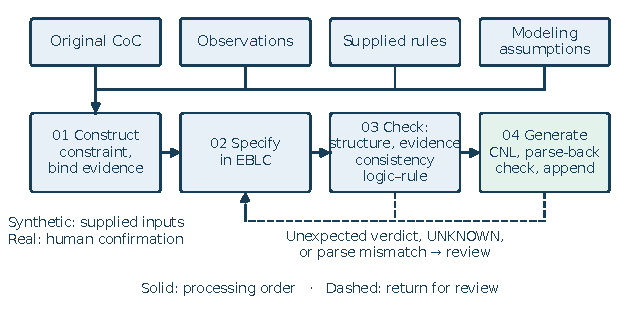
\includegraphics[width=\linewidth]{figures/method-flow.pdf}
\caption{GuardSynth workflow. Four inputs feed four stages. Unexpected
solver verdicts, UNKNOWN, or a sentence-parsing mismatch return the
specification for review. Synthetic experiments use supplied inputs; real
scenes require human confirmation of applicability. In the reported
experiments, evidence and sentence correspondence were assessed after training
(Section~\ref{sec:method-checks}).}
\label{fig:method-workflow}
\end{figure}

\subsection{Constraint Construction and Evidence Binding}\label{sec:method-evidence}

CoC combines observations with a causal explanation; a behavioral constraint
is a separate element that determines which actions are permitted under
specified conditions. A selection objective expresses preferences among
permitted actions.

Constraint construction identifies the applicable situation, the restricted
action, and its bound or release condition. The required information is
associated with one of the three roles in Table~\ref{tab:method-evidence}.

\begin{table}[tbp]
\caption{Roles of information used to construct a constraint}
\label{tab:method-evidence}
\small
\begin{tabularx}{\linewidth}{@{}>{\raggedright\arraybackslash}p{0.19\linewidth}>{\raggedright\arraybackslash}X>{\raggedright\arraybackslash}X@{}}
\toprule
Role & Example & Use in interpretation\\
\midrule
Observation & Time at which the pedestrian leaves the conflict zone & Supplies environmental state and event time\\[3pt]
Supplied rule & Wait at least 0.5 s after clearance & Determines the temporal boundary of admissibility\\[3pt]
Modeling assumption & No reoccupation after clearance & Defines the scope of the temporal interpretation\\
\botrule
\end{tabularx}
\end{table}

This separation distinguishes observed facts from required behavior. Clearance
time can be observed, but the required wait is determined by a separate rule.
Waiting durations and permitted distances are therefore taken from supplied
rules rather than inferred from video or CoC wording.

Conditions and values are linked to their supporting records, as illustrated
in Table~\ref{tab:method-specification}. If a constraint is wrong, these links
identify the observation, rule, or assumption requiring review. Recording a
source does not establish that the source is correct.

In the synthetic experiments, the generator supplies observations, rules, and
candidate measurements to predefined specification constructors. The original
natural-language CoC is retained; these experiments do not parse its unrestricted
meaning into EBLC. Real-scene use requires human confirmation of the
relevant entities, regions, event times, and rule applicability. Automatic
extraction of this information from video and its quality are not evaluated
in this study.

\subsection{EBLC Specifications}\label{sec:method-eblc}

An Evidence-Bound Lifecycle Contract (EBLC) records a behavioral constraint
through its subject and target, applicability, action restriction, persistence
and release, time and units, and supporting evidence and assumptions.
``Evidence-bound'' denotes the connection between values and their source
records. ``Lifecycle'' covers activation, persistence, release, and, where
needed, reactivation. Each task uses the required elements; only combinations
supported by the validator and logical interpretation are accepted.

\noindent\textbf{Pedestrian-entry constraint.}
This constraint prohibits entry while the conflict zone is occupied and
requires a specified wait after clearance. Table~\ref{tab:method-specification}
shows the semantic contents of its specification for a 0.5 s rule and of the
position-hold specification described below, without
implementation identifiers, together with the CNL phrase generated from each
element.

\begin{table}[tbp]
\caption{EBLC specifications and the CNL phrase generated from each element}
\label{tab:method-specification}
\footnotesize
\begin{tabularx}{\linewidth}{@{}>{\raggedright\arraybackslash}p{0.17\linewidth}>{\raggedright\arraybackslash}p{0.24\linewidth}>{\raggedright\arraybackslash}p{0.15\linewidth}>{\raggedright\arraybackslash}X@{}}
\toprule
Element & Value & Role & Generated phrase\\
\midrule
\multicolumn{4}{@{}l}{\textit{Pedestrian entry, 0.5 s wait}}\\[2pt]
Subject and target & Ego vehicle; pedestrian conflict zone & Restriction scope & ``the pedestrian conflict zone''\\[3pt]
Restricted action & No entry during occupancy & Action restriction & ``Do not enter \ldots\ while it is occupied.''\\[3pt]
Release requirement & At least 0.5 s of clearance & Supplied rule & ``Enter only after the zone has remained clear for at least 0.5 s.''\\[3pt]
Assumption & A single clearance transition with no reoccupation & Interpretation scope & Not rendered\\[3pt]
Evidence & Supplied synthetic rule and its source-record identifiers & Traceability & Not rendered\\
\midrule
\multicolumn{4}{@{}l}{\textit{Position hold, 2.0 s}}\\[2pt]
Subject and target & Ego vehicle; initial XY position & Restriction scope & ``the ego vehicle's initial position''\\[3pt]
Hold duration & 2.0 s & Supplied rule & ``Hold \ldots\ for at least 2.0 s.''\\[3pt]
Checked samples & Listed waypoints with $t\le2.0$ s, endpoint included & Interpretation scope & ``At every listed waypoint with t <= 2.0 s, including the endpoint,''\\[3pt]
Restricted action & Radial distance at most 0.2 m & Action restriction & ``the radial XY distance from the initial position must be at most 0.200 m.''\\[3pt]
Release & Motion permitted after the hold & Release & ``Movement after that period is permitted.''\\[3pt]
Assumption & Waypoints relative to the initial origin & Interpretation scope & Stated in candidate descriptions\\[3pt]
Evidence & Supplied synthetic rule and its source-record identifiers & Traceability & Not rendered\\
\botrule
\end{tabularx}
\end{table}

Clearance time is an observation supplied during checking, not a value stored
in this specification. Let $\tau$ be clearance time, $u$ the candidate's entry
time, $\Delta$ the required wait, and $e$ its Boolean entry flag. Under the
no-reoccupation assumption, admissibility requires
\begin{equation}\label{eq:method-entry}
e\Rightarrow u\ge\tau+\Delta.
\end{equation}
The specification supplies $\Delta$, whereas the environment and candidate
supply $\tau$, $u$, and $e$. This separation permits different rules to be
applied to the same environment and different candidates to be checked against
the same specification.

For example, clearance at 11.0 s permits entry from 11.5 s under a 0.5 s rule
and from 12.5 s under a 1.5 s rule. The scene and candidates can be identical
while the admissible set changes. A non-entry candidate satisfies both rules;
its selection depends on progress.

\noindent\textbf{Position-hold constraint.}
This constraint requires a candidate to stay within a permitted radius of its
initial position for a specified duration. Let $T$ be the hold duration, $R$
the permitted radius, and $(x_i,y_i)$ the candidate's sampled coordinates
relative to its initial position. Admissibility requires
\begin{equation}\label{eq:method-hold}
\bigwedge_{t_i\le T}\left(x_i^2+y_i^2\le R^2\right).
\end{equation}
We use $R=0.2\,\mathrm{m}$ and $T\in\{0.5,2.0\}\,\mathrm{s}$. The interval
includes its endpoint; movement after the hold period is unrestricted. Only
the listed samples are checked, rather than continuous motion between samples
or vehicle dynamics.

The same candidates are presented in two forms. \textbf{Time-indexed XY
coordinates} require the model to identify samples within the hold interval
and assess their distances from the initial position. \textbf{Interval maxima}
supply every candidate with both $D_{\max}(0.5\,\mathrm{s})$ and
$D_{\max}(2.0\,\mathrm{s})$, where
$D_{\max}(T)=\max_{t_i\le T}\sqrt{x_i^2+y_i^2}$, regardless of the active
rule; the model must still select the required interval and compare its
maximum with the permitted radius. Reference admissibility is computed from
the original integer coordinates and squared distances, not rounded maxima
displayed in the prompt. Comparing the two forms helps distinguish
coordinate-calculation demands from constraint-based selection, although it
also changes the input representation.

\noindent\textbf{Numerical bounds.}
Speed, clearance, and entry-delay tasks place an upper or lower bound on a
candidate measurement. With completion flag $q$, measurement $x$, and bound
$b$, the basic form is
\begin{equation}
q\Rightarrow(x\ \mathrm{op}\ b),\qquad
\mathrm{op}\in\{\le,\ge\}.
\end{equation}
Section~\ref{sec:method-cnl} explains the treatment of non-completing
candidates and its difference from the generated language.

\noindent\textbf{Activation, persistence, and release.}
The preceding constraints are evaluated from supplied values. A separate
qualitative specification tracks obligations when evidence changes over time:
valid activation or release evidence updates the state, while uncertain or
conflicting evidence preserves the previous state. Its state-transition checks
are reported in Supplementary Section S3; the learning experiments
do not use this specification.

Table~\ref{tab:method-tasks} connects each task to its admissibility condition.
The first six tasks form the six-task comparison; position holding is evaluated
in both the fresh-adapter and continuation studies. All numerical bounds are
supplied experimental rules. Entry delay $\delta$ is a duration, whereas $u$ is an instant. In stopping,
$o$ is position relative to the stop line, with negative values before the
line; $a_{\mathrm{peak}}$ and $j_{\mathrm{peak}}$ denote peak deceleration and jerk.

\begin{table}[tbp]
\caption{Task admissibility conditions with representative supplied rules.
$q$ denotes completion and $e$ denotes entry.}
\label{tab:method-tasks}
\small
\begin{tabularx}{\linewidth}{@{}>{\raggedright\arraybackslash}p{0.22\linewidth}>{\raggedright\arraybackslash}X@{}}
\toprule
Task & Admissibility condition\\
\midrule
Maximum speed & $q\Rightarrow v\le4.4\,\mathrm{m/s}$\\[4pt]
Minimum clearance & $q\Rightarrow d\ge2.0\,\mathrm{m}$\\[4pt]
Minimum entry delay & $q\Rightarrow\delta\ge2.5\,\mathrm{s}$\\[4pt]
Pedestrian entry & $e\Rightarrow u\ge\tau+\Delta$\\[4pt]
Stopping & $q\Rightarrow(o\le0\land a_{\mathrm{peak}}\le5.8\,\mathrm{m/s^2}\land j_{\mathrm{peak}}\le7.4\,\mathrm{m/s^3})$\\[4pt]
Lane change & $q\Rightarrow g\ge5.8\,\mathrm{m}$\\[4pt]
Position holding & $\displaystyle\bigwedge_{t_i\le T}(x_i^2+y_i^2\le R^2)$\\
\botrule
\end{tabularx}
\end{table}

\subsection{Specification Checking}\label{sec:method-checks}

The admissibility conditions in Section~\ref{sec:method-eblc} are translated
into logical formulas. We use SMT and
Z3~\cite{r11,r12} and distinguish property queries from candidate queries.
The learning specifications are evaluated through satisfiability, candidate
admissibility, and concrete logic--rule comparisons. Property-query semantics
are illustrated below; the separate qualitative lifecycle example in
Supplementary Section S3 is not used for learning.

\noindent\textbf{Specification properties.}
Let $\Phi$ combine the specification and its assumptions, and let $P$ be a
property of interest. The counterexample query is
\begin{equation}
\Phi\land\neg P.
\end{equation}
UNSAT means that no counterexample exists within the encoded scope. SAT means
that an assignment satisfies the specification while violating the property.
Because an inconsistent specification implies every property vacuously, the
satisfiability of $\Phi$ is checked separately.

For the entry constraint, the requirement that entry occur only after the
release boundary can be expressed as $P=(e\Rightarrow u\ge\tau+\Delta)$.
Its counterexample query, $\Phi_C\land e\land(u<\tau+\Delta)$, must be UNSAT.
Removing the release restriction permits a SAT counterexample. This illustrates
property-query semantics; the fault-injection logic--rule comparisons below use
concrete boundary assignments.

\noindent\textbf{Candidate queries.}
Let $B(a)$ fix candidate $a$'s measurements and completion or entry flag. We
check
\begin{equation}
\Phi_C\land B(a).
\end{equation}
SAT means that the candidate is compatible with the constraint, and UNSAT means
that it is incompatible. This query checks admissibility, not whether the
candidate is the preferred one.

Before training, the pedestrian-entry and position-hold specifications used for
learning underwent structural validation, satisfiability checks, and candidate
checks.

\noindent\textbf{Checking layers.}
Five checks compare different objects.
\begin{enumerate}
\item \textbf{Structural check:} verify supported field combinations, values,
and units.
\item \textbf{Satisfiability check:} confirm that the base specification is
satisfiable, so that properties do not hold vacuously.
\item \textbf{Logic--rule comparison:} compare logical verdicts for concrete
candidates with verdicts computed by independent integer rules from the
supplied rule. Archived action candidates are evaluated together with boundary
probes: for pedestrian entry, entry or non-entry at $-1,0,+1$ ms around release;
for position holding, distances of 199, 200, and 201 mm, with diagonal norm
checks, at every listed non-initial sample, including samples after release.
The 1 ms spacing tests logical boundaries, not vehicle-control precision.
\item \textbf{Evidence correspondence check:} compare the specification with
the supplied rule record.
\item \textbf{Sentence correspondence check:} parse the generated CNL with a
fixed grammar for the specification, reconstruct the supported fields, and
compare them with the original specification.
\end{enumerate}
Evidence correspondence, sentence correspondence, and boundary probes for
logic--rule comparison were added for the fault-injection evaluation below;
they were not applied in the reported training runs.

\noindent\textbf{Fault-injection evaluation.}
To assess which check detects which error, we inject faults into the
pedestrian-entry and position-hold specifications used to produce learning
inputs. Each task contributes 24 base cases: 12 archived evaluation contexts
paired with two supported durations (0.5/1.5 s for entry and 0.5/2.0 s for
holding). These are repeated contexts under two rule settings, not 24 distinct
specification parameterizations or independent road scenes. Before injection,
we verify the archived specifications and P2 text against the maintained
constructors and renderers. The evaluation reuses the unaltered structural
validators, logical lowering, renderers, and SMT compiler.

Each base case yields one valid case, six supported faults, and one control in
which the source record and the specification are changed to the same wrong
value: 192 cases per task and 384 in total. The faults change a supported
duration in the specification only, reverse a comparison, omit a release
condition, change a unit without rescaling, or alter the sentence's duration
or negation. For entry, release omission removes the entry gate. For holding,
it keeps the distance restriction active after the hold ends, and comparison
reversal affects the inclusive hold endpoint. The probes comprise 7,392
concrete queries; UNKNOWN outcomes are recorded separately. Detection results
are reported in Section~\ref{sec:results-checks} (Table~\ref{tab:results-faults}).

Sentence correspondence is limited to each specification's fixed grammar.
Fixed patterns constrain the target, units, negation, and relation; the parser
extracts the duration and reconstructs the supported fields. This is not a
general test of semantic equivalence for arbitrary language. An earlier
fault-injection evaluation on a separate pedestrian-entry specification,
developed for the expression-diversity study, uses probes at $-100,0,+100$ ms
(192 cases) and is described in Supplementary Section S4.

\noindent\textbf{Scope of the checks.}
Check conclusions hold only within supported specification structures,
supplied inputs, explicit assumptions, and the finite logical scope. The
accident examples in the Introduction motivate checking interacting
requirements, but the reported experiments assess the supported task
specifications rather than reconstructing those accidents or verifying a
general composition of traffic rules and vehicle dynamics. Consistency of a
specification alone does not establish safe behavior or progress toward an
objective. Pedestrian entry assumes a single clearance transition without
reoccupation; position holding checks only listed coordinate samples.
Evidence records and internal consistency do not establish observation truth,
rule suitability, or road safety, and logic--rule comparison establishes
correspondence between two implementations of the same supplied rule.

Specification checking and model evaluation measure different objects. The
former assesses correspondence among structure, evidence, logic, and language;
the latter measures whether the selected candidate is admissible and
preferred. A model can select a prohibited candidate even when its
specification passes the checks, so Section~\ref{sec:results} reports the two
with their respective evaluation units and denominators.

\subsection{Composition of Supplied Constraints}\label{sec:method-composition}

The composition diagnostic checks whether separately supplied conditions can
hold together under an explicit shared context. Let $\Phi_E$ encode supplied
observations and modeling assumptions, and let $\Phi_j$ encode source
constraint $j$. For a selected source set $\Gamma$, the query is
\begin{equation}
\Phi_E\land\bigwedge_{j\in\Gamma}\Phi_j.
\end{equation}
SAT provides an assignment satisfying the selected conditions together;
UNSAT identifies an incompatible combination relative to $\Phi_E$. The context
is checked first. Every source constraint is then checked separately, in pairs,
and in the full combination. Enumerating subsets for these two- or three-source
cases identifies subset-minimal conflict groups: the group is UNSAT and every
proper subset is SAT. This identifies incompatible requirements, not which
source should be changed.

Documented conditions are kept separate from authored states, candidate
requests, modeling assumptions, and test objectives. We manually reviewed
official accident investigations, operating guides, traffic guidance, and
regulations; the selected cases use NTSB, FHWA, Waymo, and UK Department for
Transport documents. The constraints are manually formalized, then executed
by the unchanged platform Core/SMT compiler. Supplementary Section S13 lists every natural-language statement
with its source role and formal condition; these statements explain the
formalization and are not outputs of an unrestricted parser or the CNL
correspondence evaluation.

The braking case selects the historical suppression branch with an already
recognized emergency, persistent hazard, no takeover, and no alternative
path~\cite{NTSB2019Tempe}. The NTSB policy record gives a braking delay
$t_b\ge1$ s; an authored constant-deceleration model gives stopping distance
$x\ge vt_b+v^2/(2a)$; and an authored test objective requires $x\le d$.
Emergency-trigger eligibility and jerk are outside the model, and the
authored terms determine whether the selected delay is compatible with a
hypothetical state. The signal case uses FHWA's nominal stopping
model and a two-action stop/proceed abstraction~\cite{FHWA2009Yellow,FHWA2008Timing}.
The interlock case checks candidate autonomous driving against the
manufacturer's listed blockers~\cite{Waymo2026Emergency}; it makes no claim
about rolling or towing. The Rule 129 case fixes other exceptions absent
and compares a restricted faithful encoding with a deliberately omitted
stationary-vehicle exception~\cite{DfT2015HighwayCode129}.

Candidate requests are explicit: permission to cross does not require
crossing, and a blocked driving candidate does not make holding inconsistent.
These distinctions prevent manufactured conflicts from turning optional
progress into an unconditional obligation. The diagnostic checks
compatibility within the stated abstractions, rather than reconstructing
accidents or establishing the safety of an operating system or a complete
operating policy. Supplementary Section S13 retains the earlier synthetic
boundary diagnostic separately.

\subsection{Language Generation and CoC Augmentation}\label{sec:method-cnl}

CNL is generated only from structurally validated specifications. Fixed
sentence rules express the target, restricted action, condition, value, and
unit. Neither reference labels nor progress scores are inputs to the renderer.
The pedestrian-entry specification with a 0.5 s wait generates:
\begin{quote}\small
Do not enter the pedestrian conflict zone while it is occupied. Enter only
after the zone has remained clear for at least 0.5 s.
\end{quote}
The first sentence expresses the occupancy prohibition; the second expresses
the release and waiting condition (Table~\ref{tab:method-specification}). ``At least''
includes the boundary, and ``only after'' states a necessary condition for
entry rather than an instruction to enter at a particular time.
Generated sentences follow the original CoC, before candidate descriptions and
the selection instruction. Fig.~\ref{fig:method-inputs} reproduces two complete
model inputs. Clearance time is supplied separately, so this text does not give the answer
time directly. The EBLC specification, check verdicts, and evidence records
are not inserted into the model prompt.

\begin{figure}[tbp]
\centering
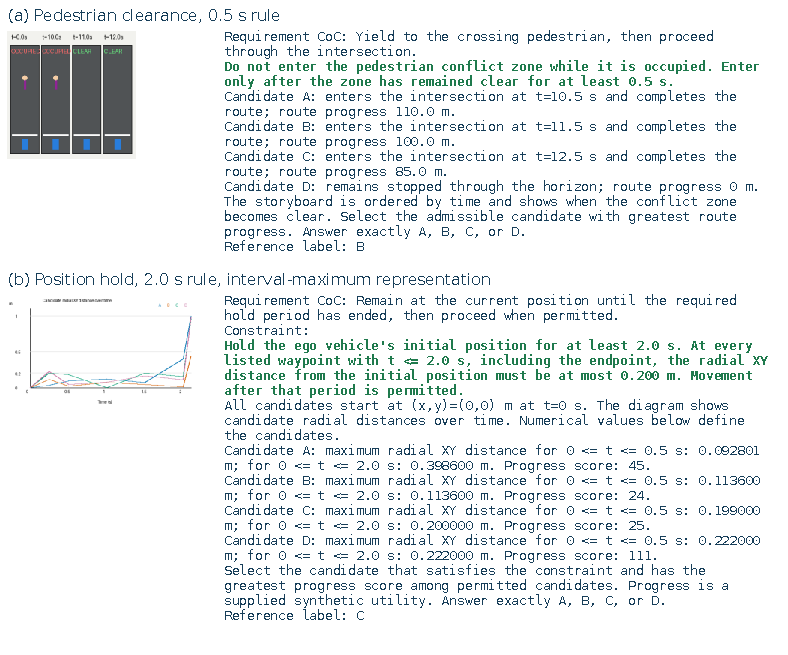
\includegraphics[width=\linewidth]{figures/input-examples.pdf}
\caption{Two archived test inputs. (a) Pedestrian entry with a 0.5 s rule.
(b) Position hold with a 2.0 s rule and interval-maximum candidate
descriptions. Bold green text is the CNL generated from an EBLC specification
(P2); P0 inputs omit it. Text is verbatim except for line breaks added around
the CNL. The model outputs one candidate label; the reference label is shown
for illustration and is not part of the input.}
\label{fig:method-inputs}
\end{figure}

\noindent\textbf{Comparison conditions.}
P0 uses the original CoC, P1 adds a directly written natural-language guard,
and P2 adds CNL generated from an EBLC specification. For pedestrian entry, P1 uses a
template from the preceding study that produces language directly from rule
values~\cite{r4}:
\begin{quote}\small
Do not enter while the pedestrian conflict zone is occupied. After it becomes
clear, remain stopped for at least 0.5 s before entering.
\end{quote}
The temporal candidates specify entry times or non-entry, so P1 and P2 induce
the same admissible set in this task. However, ``remain stopped'' is stronger:
it also restricts motion without entry. We do not claim equivalence for general
trajectories.

For position holding, the original CoC is:
\begin{quote}\small
Remain at the current position until the required hold period has ended, then
proceed when permitted.
\end{quote}
Its P1 natural-language guard uses a template written for this task:
\begin{quote}\small
For the first 2.0 seconds, keep the vehicle within 0.200 metres of its starting
point at all listed times, including the final time of this waiting period.
Moving farther away is allowed only after this period ends.
\end{quote}
Its P2 sentences are generated from the position-hold specification
(Table~\ref{tab:method-specification}; Fig.~\ref{fig:method-inputs}b).
P1 and P2 share a learning interface; their comparison examines differences
in wording and construction path. Rule availability in each study is
summarized in Table~\ref{tab:setup-comparisons}.

\noindent\textbf{Scope of sentence correspondence.}
The logical conditions for static and maneuver tasks do not classify
non-completing candidates as violations, but their generated sentences do not
express this exemption. Sentence--logic correspondence in these tasks is
therefore limited to numerical bounds for completing candidates.

% project_id: guardsynth-coc
\noindent\textbf{Use of AI-assisted tools.}
OpenAI Codex was used to assist with English translation and revision of the
manuscript and with implementation and checking of supporting scripts. The
authors retain responsibility for the scientific content, analyses, and final
manuscript. This assistance is separate from the Qwen and Alpamayo models
evaluated in the experiments.


% !TeX root = ncaa-manuscript-en.tex
\section{Experimental Setup}\label{sec:experimental-setup}

This section defines two evaluation tracks: constraint compliance and preferred
candidate selection by the model, and checking the specifications used to
construct learning inputs. It defines the tasks and reference labels, the
metrics and aggregation units, and the training and comparison protocols.
All learning experiments use synthetic candidate selection; the protocol of
the preliminary Alpamayo-R1 diagnostics is given in Supplementary Section S1.

\subsection{Tasks and Data}\label{sec:setup-data}

Each example contains an image, the original CoC, a constraint sentence when
provided by the condition, descriptions of the supplied candidates, and a selection
instruction (Fig.~\ref{fig:method-inputs}). Candidate measurements are supplied
in text; the VLM does not estimate them from the image. Static tasks have two
candidates; pedestrian entry, maneuver tasks, and position holding have four.

\noindent\textbf{Six behavioral tasks.}
The six tasks form three families. Static tasks apply maximum-speed,
minimum-clearance, and minimum-entry-delay rules to numerical candidate
summaries. Pedestrian-entry examples vary the clearance time, required wait,
candidate entry times, and label assignments. Maneuver tasks concern stopping
and lane changing. Examples occur in pairs with the same scene and candidates
but different supplied rules, so the preferred candidate can change: entry 0.5 s
after a zone clears is admissible under a 0.5 s waiting rule but prohibited
under a 1.5 s rule.

\noindent\textbf{Position holding.}
This task uses the position-hold constraint in Section~\ref{sec:method-eblc}. Synthetic
candidate profiles are presented as XY coordinates or as interval-maximum
distances calculated from the same coordinates; images are diagrams of the
profiles. Each profile yields eight rows: two label rotations, two hold
durations, and two representations. The training, validation, and test splits
contain 120, 16, and 32 profiles, with no profile shared across splits.

Table~\ref{tab:setup-dataset-sizes} gives rows per input condition. P0, P1, and
P2 share examples and splits, differing only in their constraint text. Rows are
constructed examples rather than independent road videos. Pedestrian-entry
images do not overlap across splits, whereas all 13 static primary-test images
also occur in training and maneuver data reuse two diagrams. Static and
maneuver results therefore measure the use of supplied constraints rather than
visual generalization. Split inventories are given in Supplementary Section S2.

\begin{table}[tbp]
\caption{Synthetic dataset sizes per input condition. A dash denotes no
separate validation split.}\label{tab:setup-dataset-sizes}
\centering
\small
\begin{tabular*}{\textwidth}{@{\extracolsep\fill}lrrr@{}}
\toprule
Task family & Training & Validation & Primary test\\
\midrule
Pedestrian entry & 960 & 240 & 240\\
Static (three tasks) & 576 & -- & 144\\
Maneuver (two tasks) & 384 & -- & 96\\
Position hold & 960 & 128 & 256\\
\botrule
\end{tabular*}
\end{table}

\noindent\textbf{Preferred candidates and reference labels.}
As defined in Section~\ref{sec:method-problem}, the preferred candidate has the
highest supplied progress score among admissible candidates; its label is the
reference label. Admissibility is computed from the
supplied rule and candidate values by integer calculations implemented
separately from the logical encoding; position holding checks
$x_i^2+y_i^2\le 200^2$ (mm) for every sample up to the hold endpoint. SMT
candidate verdicts are compared with these calculations
(Section~\ref{sec:results-checks}) and kept as metadata rather than placed in
the prompt. The
supervised response contains only the reference label. Progress scores are
supplied synthetic values whose ordering among admissible candidates
determines the preferred candidate. Labels rotate within each task's label
set: A--B for static tasks and A--D for the other tasks (Supplementary Section S2). Score variation and label rotation reduce fixed
associations between the answer and a label, position, or score, but do not
remove shortcuts based on the supplied numerical values.

\subsection{Metrics and Aggregation}\label{sec:setup-metrics}

\noindent\textbf{Preferred-selection score (PSS)} assigns one to a prediction
that selects the reference label of the highest-scoring admissible candidate,
and zero to every other output. The mean is reported as a percentage. It
measures how often the preferred candidate is selected, not the size of the
progress-score difference when another candidate is selected.
\textbf{Constraint violation rate (CVR)} is the percentage of all predictions
that select a prohibited candidate. An admissible candidate with a lower
progress score receives zero for preferred selection but is not a violation.
The two metrics therefore need not sum to 100\%.
\textbf{Rule-pair accuracy (RPA)} is the percentage of same-scene,
same-candidate pairs with different supplied rules for which both reference
labels are selected. Some position-hold pairs share a reference label, so
this metric does not require a changed choice in every pair.
\textbf{Constraint-compliant completion} is the percentage completing the task without
selecting a prohibited candidate; it is auxiliary. Unextractable answers
receive zero preferred-selection credit and count as neither violations nor
admissible choices; their rate is reported separately. Thus, the complement of the
constraint violation rate is not the admissible-choice rate when extraction
failures occur. Position-hold violations use the strict 0.2 m radius, with a
0.01 m tolerance reported only as an auxiliary measure.

Reported seed standard deviations use the sample convention ($n-1$).
Fresh-adapter results report means and sample standard deviations
over three seeds. Each condition combines both durations, yielding 720
pedestrian-entry predictions (240 rows $\times$ three seeds) or 384
position-hold predictions per representation (128 rows $\times$ three seeds).
Continuation results report counts per duration and
representation (192 predictions from 64 rows and three seeds). Six-task and
additional evaluations report three-seed means. Supplementary Section S6 gives
individual seeds for the fresh-adapter, six-task, representation, and robustness
comparisons; reasoning-prompt and exploratory diagnostics are detailed in
Supplementary Sections S8 and S10. Seeds repeat optimization and do not add
independent examples.

Specification checks comprise the fault-injection evaluation of
Section~\ref{sec:method-checks} (384 cases, 7,392 queries), the 5,376
position-hold candidate checks, and, for the pedestrian-entry specification,
one satisfiability query and 24 boundary-candidate queries for each of four
waits (0.5, 1.5, 0.8, and 1.8 s), 100 queries in total. These units are
reported separately from each other and from model-prediction denominators.
\subsection{Model and Training Settings}\label{sec:setup-training}

We fine-tune Qwen3-VL-2B-Instruct~\cite{qwen2025qwen3vl2b}, a model small
enough for every comparison to be repeated with fresh adapters over three seeds
under matched budgets; a larger model of the same family is evaluated without
training (Section~\ref{sec:setup-comparisons}). Adaptation uses
LoRA~\cite{r14} (rank 8, $\alpha=16$, dropout 0.05) with AdamW (learning rate
$2\times10^{-4}$, weight decay 0.01), batch size 2, and gradient accumulation
over eight steps. Each fit runs for three epochs with optimization seed 42, 17,
or 123; pedestrian-entry and position-hold fits perform 180 updates, and static
and maneuver fits 108 and 72. Within each task family, compared conditions
share examples, epochs, optimizer settings, and the final-checkpoint policy;
validation scores do not select checkpoints. Input lengths differ across text
conditions. Fine-tuned adapters use greedy decoding with a 12-token answer
limit.

\subsection{Comparison Designs}\label{sec:setup-comparisons}

Table~\ref{tab:setup-comparisons} distinguishes three studies by the information
available during training and evaluation. Models trained with constraint text
also receive it at evaluation, matching the intended use of case-specific
constraints (Section~\ref{sec:discussion-training}).

\begin{table}[tbp]
\caption{Training and evaluation information in the three studies. Fresh
adapters share their initialization within each task and seed.}
\label{tab:setup-comparisons}
\footnotesize
\begin{tabularx}{\textwidth}{@{}>{\raggedright\arraybackslash}p{0.14\textwidth}>{\raggedright\arraybackslash}X>{\raggedright\arraybackslash}X>{\raggedright\arraybackslash}X@{}}
\toprule
Study & Training & Evaluation & Question\\
\midrule
Fresh-adapter study & Same pretrained base; CoC alone or CoC + CNL, each with or
without semantic loss & (a) Training input type; (b) same CoC + CNL for all
adapters & With evaluation information and initialization held fixed, do
training constraints reduce violations and improve rule-dependent selection?\\[4pt]
Continuation study & Existing pedestrian-entry adapters; P0: CoC,
P1: CoC + natural-language guard, P2: CoC + CNL & Same CoC + P2 CNL for every
adapter, before and after continuation & Does a constraint-bearing training
history improve behavior under identical evaluation inputs?\\[4pt]
Six tasks & P0: CoC; P1 and P2: CoC + respective constraints & Same input type
as training & Do models use supplied constraints and change their choices when
the rule changes?\\
\botrule
\end{tabularx}
\end{table}

\noindent\textbf{Fresh-adapter study.}
We train new LoRA adapters from the same pretrained base on pedestrian entry and
position holding. The $2\times2$ design crosses CoC-only versus CoC + CNL inputs
with cross-entropy (CE) alone versus CE plus semantic loss; seed-specific
initial LoRA tensors are identical across the four conditions. Two tasks, four
conditions, and three seeds yield 24 fits. Our semantic loss is a categorical
adaptation of Xu et al.~\cite{Xu2018}. At the first supervised answer-token
position, let $z_a$ be the logit for label $a\in\mathcal{Y}=\{A,B,C,D\}$:
\begin{equation}\label{eq:setup-semantic-loss}
q_a=\frac{\exp z_a}{\sum_{b\in\mathcal{Y}}\exp z_b},\qquad
\mathcal{L}_{\mathrm{train}}=\mathcal{L}_{\mathrm{CE}}
-\lambda\log\!\sum_{a\in\mathcal{Y}_C}q_a,
\end{equation}
where $\mathcal{Y}_C\subseteq\mathcal{Y}$ is the set of labels whose candidates
are admissible. We fix $\lambda=1$ before execution. Even with CoC-only inputs,
the loss uses the example's admissible set, so rule information enters through
the objective; inference neither filters candidates nor uses SMT. The protocol
specifies evaluation with the training input type as primary and common-CNL
evaluation as additional; we report both and emphasize the latter when
comparing training conditions.

\noindent\textbf{Continuation study.}
We continue the nine pedestrian-entry adapters (P0, P1, P2 $\times$ three
seeds) on 960 position-hold rows for 180 further updates. P0 receives the
original CoC at both stages, while P1 and P2 receive their respective
constraints at both stages. Before and after continuation, all adapters
receive identical inputs with the P2 constraint sentence. The comparison
therefore includes the effects of different training histories. Previously
inspected profiles with prohibited candidates only 1 mm beyond the radius are
reevaluated separately as a regression check (Supplementary Section S11).

\noindent\textbf{Identifiability without rule text.}
When the distinguishing rule is omitted, identical inputs can have different
reference labels. Every six-task rule pair has different reference labels, giving a
50\% preferred-selection score ceiling for rule-free inputs; in the position-hold set, half the
pairs do, giving an empirical ceiling of 75\%. Fewer violations without rule
text therefore do not show that a model changes its choice with the rule, and
the six-task study measures the use of constraints supplied at both training
and evaluation rather than a training benefit under identical information.
Rule-pair accuracy and the common-CNL evaluation are used for this reason to
assess rule-dependent selection directly.

\noindent\textbf{Pretrained-VLM evaluation.}
Qwen3-VL-2B-Instruct and Qwen3-VL-8B-Instruct~\cite{qwen2025qwen3vl2b,qwen2025qwen3vl8b}
receive CoC and CNL without fine-tuning or demonstrations on all 736
primary-test inputs, with one greedy response per input. The primary evaluation
fixes a 12-token output limit before execution; after observing truncated
explanations, we add a post-hoc evaluation with a 512-token limit and
final-answer extraction, and report both, together with output-limit hits and
answer-extraction failures. This comparison includes adaptation
to the task format and is not a matched-budget training comparison.

\subsection{Comparison Conditions and Related Approaches}\label{sec:setup-related}

The systems reviewed in Section~\ref{sec:related-work} use different
interfaces: DriveLM and DriveVLM address driving question answering and
planning, while nl2spec and NL2TL output temporal-logic formulas rather than
action labels~\cite{r2,r3,r8,r9}. Their native execution paths are documented
in Supplementary Section S5; adding our constraints or an output adapter would
evaluate modified methods. We instead use controls that share selected
principles with prior work (Table~\ref{tab:setup-related-controls}); they are
not reproductions of the cited systems.

\begin{table}[tbp]
\caption{Comparison conditions and principles shared with related approaches.
Correspondences identify selected principles, not reproductions of complete
systems.}\label{tab:setup-related-controls}
\footnotesize
\begin{tabularx}{\textwidth}{@{}>{\raggedright\arraybackslash}X>{\raggedright\arraybackslash}X>{\raggedright\arraybackslash}p{0.25\textwidth}@{}}
\toprule
Condition & Shared principle & Budget\\
\midrule
CNL at evaluation for CoC-only-trained adapters & Use of rules at inference;
regulation-augmented reasoning also uses rules at this stage~\cite{r7} &
Matched fresh-adapter training; continuation reported separately\\[4pt]
CoC + CNL for pretrained 8B & Prompting a larger model with rules & No
task-specific training\\[4pt]
Categorical semantic loss & Constraints in the training objective~\cite{Xu2018}
& Matched fresh-adapter training\\[4pt]
General reasoning prompts & Zero-shot CoT and Plan-and-Solve~\cite{r16,r17}
& No additional training; unequal generation limits\\[4pt]
Logical-text control & Formal representation of requirements~\cite{r8,r9}
& Matched pedestrian-entry training\\[4pt]
P1 and alternative natural-language guards & Natural-language constraints in
training~\cite{r4} & Matched within each task family\\
\botrule
\end{tabularx}
\end{table}

\subsection{Additional Evaluations}\label{sec:setup-additional}

The following evaluations use archived checkpoints, including those from
additional conditions trained with matched task-family budgets. Their rows are
not added to the primary-test denominator. Procedures are detailed in
Supplementary Sections S2, S8, and S10.
\begin{itemize}
\item \textbf{General reasoning prompts.} Zero-shot CoT (128 reasoning tokens)
and basic Plan-and-Solve (256 tokens)~\cite{r16,r17} are applied to the final
P0 checkpoints without rule information or further training. A first stage
generates reasoning for each unique input (546 per method), and a second stage
extracts the label; each method yields 1,440 predictions over three seeds.
\item \textbf{Paraphrasing.} A held-out constraint wording is given to P1 and
P2 on the 240, 144, and 96 primary-test rows of the three families; P0
inputs, which contain no constraint text, are unchanged. A smaller exploratory
diagnostic tests a second wording with 24 rows per wording and seed.
\item \textbf{Unseen values.} Values and durations absent from training are
used, such as pedestrian-entry waits of 0.8 and 1.8 s instead of 0.5 and 1.5 s.
\item \textbf{Combined difficulty.} A 96-row maneuver set combines negation,
clause order, equality boundaries, and m/cm units.
\item \textbf{Alternative pedestrian-entry representations.} We report two
additional conditions trained with the same budget as P0--P2: an alternative
natural-language guard and a logical formula supplied as text. Each was evaluated on the 240 primary-test
and 240 unseen-wait rows. The logical text is a model input, not a solver or
translator output.
\item \textbf{Image interventions.} Pedestrian-entry adapters receive original,
blank, or redrawn images with clearance 1.0 s later, with all other inputs and
the original references fixed (24 rows per condition, 648 predictions). Scores
on redrawn images measure an input intervention rather than scene-understanding performance;
we also report the fraction of choices that change relative to the original
image.
\end{itemize}

\subsection{Bounded Constraint-Composition Diagnostic}\label{sec:setup-composition}

This diagnostic, run after and independently of the training runs, evaluates the manually formalized
source groups in Section~\ref{sec:method-composition}. A source catalog records
the document version, URL, paragraph or page, supported interpretation, and
scope. Eight official documents were inspected; two further UNECE candidates
were excluded because their full official text could not be retrieved.
The executed cases use four document families, with scenario states,
candidate requests, motion assumptions, and test objectives marked as authored
inputs. No operational log is used.

Parameter grids bracket each feasibility threshold by 1 mm: braking (48
cases; speeds of 10/15/20 m/s, decelerations of 5/7 m/s$^2$, and delays of
0/1000 ms, with zero delay as a control), yellow-interval feasibility (64
cases; nominal deceleration of 3 m/s$^2$, not an emergency-braking bound),
all 16 interlock states with drive/hold candidates (32 cases), and all eight
exception states with cross/hold candidates and faithful/omitted-exception
encodings (32 cases). Supplementary Section S13 gives the full grids.

The 176 configurations yield 896 queries, covering the context alone and
every nonempty source subset. Verdicts are compared with independent
rational feasibility calculations, and each SAT witness is checked numerically.
For each UNSAT combination, all proper subsets identify subset-minimal
conflict groups. We distinguish incompatibility introduced by suppression
from avoidance already infeasible without it, and permission to cross from
an obligation to cross. These configurations and queries are counted
separately from fault injection, VLM predictions, and the earlier 123-case
synthetic boundary diagnostic. Supplementary Section S13 records both
protocols and their distinct scopes.


% !TeX root = ncaa-manuscript-en.tex
\section{Results}\label{sec:results}

The behavioral track first tests training with constraints under common-CNL
evaluation and training-matched evaluation
(Sections~\ref{sec:results-training} and~\ref{sec:results-semantic}), then
examines continuation training (Section~\ref{sec:results-continuation}).
The six-task and rule-pair results assess use of the supplied rule; reasoning,
wording, value, and image controls examine alternative explanations and
robustness. The specification track separately reports fault detection and
candidate-verdict correspondence (Section~\ref{sec:results-checks}). A separate diagnostic tests composition
consistency (Section~\ref{sec:results-composition}).
Section~\ref{sec:results-summary} brings the two tracks together.

Answer-extraction failures are zero in the fresh-adapter, continuation,
regression, six-task, robustness, reasoning-prompt, and exploratory
image/wording evaluations. The pretrained-model evaluations have nonzero
failure rates, reported below and in Supplementary Section S7.

\subsection{Constraint Training with Identical Evaluation Inputs}\label{sec:results-training}

The fresh-adapter study uses two evaluations: inputs matching each training
condition and a common-CNL evaluation for every adapter
(Section~\ref{sec:setup-comparisons}). This subsection emphasizes the latter,
which fixes evaluation information. Section~\ref{sec:results-semantic} reports
the same adapters with training-matched inputs, keeping the effects of input
information and loss design distinct.

\noindent\textbf{Same initialization and evaluation inputs.}
Table~\ref{tab:results-common-rule} compares the four fresh-adapter conditions;
individual-seed values are given in Supplementary Section S6. In the CE-only
comparison, the conditions differ in whether constraint sentences appear in
training. With the same CNL at evaluation, CoC-only-trained adapters violate
the rule in 17.92\% of pedestrian-entry predictions and 6.51\% and 6.25\% of
position-hold predictions with interval maxima and XY coordinates, respectively.
Training with CNL reduces these rates to 1.11\%, 0.00\%, and 1.56\%.
Preferred-selection score increases from 50.14\%, 78.39\%, and 75.52\% to 98.47\%, 96.09\%,
and 93.49\%. With initialization and evaluation information controlled, these
differences support the benefit of including constraint text during training.

\begin{table}[tbp]
\caption{Fresh adapters with identical CNL at evaluation. Cells show preferred-selection score
(first line) and constraint violation rate (second line), in percent, as mean $\pm$
standard deviation over three seeds. Column labels describe training inputs.}
\label{tab:results-common-rule}
\centering\footnotesize
\setlength{\tabcolsep}{3pt}
\begin{tabularx}{\textwidth}{@{}>{\raggedright\arraybackslash}Xcccc@{}}
\toprule
Task & \shortstack{CoC\\CE} & \shortstack{CoC\\CE + semantic} &
\shortstack{CoC + CNL\\CE} & \shortstack{CoC + CNL\\CE + semantic}\\
\midrule
Pedestrian entry & \shortstack{$50.14\pm1.46$\\$17.92\pm8.91$} &
\shortstack{$50.00\pm0.00$\\$0.00\pm0.00$} &
\shortstack{$98.47\pm1.20$\\$1.11\pm1.58$} &
\shortstack{$97.64\pm2.14$\\$0.83\pm1.44$}\\[5pt]
Position hold: maxima & \shortstack{$78.39\pm1.97$\\$6.51\pm3.52$} &
\shortstack{$75.52\pm0.90$\\$0.26\pm0.45$} &
\shortstack{$96.09\pm1.35$\\$0.00\pm0.00$} &
\shortstack{$96.09\pm2.34$\\$0.00\pm0.00$}\\[5pt]
Position hold: XY & \shortstack{$75.52\pm0.45$\\$6.25\pm2.71$} &
\shortstack{$74.74\pm0.45$\\$0.52\pm0.90$} &
\shortstack{$93.49\pm1.19$\\$1.56\pm0.78$} &
\shortstack{$92.71\pm3.61$\\$2.08\pm2.96$}\\
\botrule
\end{tabularx}
\end{table}

CoC-only-trained preferred-selection score remains close to the rule-free input ceilings of
50\% for pedestrian entry and 75\% for position holding, even after CNL is
provided at evaluation. These ceilings apply when rule text is absent
(Section~\ref{sec:setup-comparisons}); they are not mathematical upper bounds
for the common-CNL inputs. Rule-pair accuracy also separates the CE-only
conditions: CoC-only-trained adapters reach 1.94\%, 56.77\%, and 51.56\%,
whereas CNL-trained adapters reach 96.94\%, 92.71\%, and 86.98\%. In these
checkpoints, training with constraint text supports stronger rule-dependent
selection than inference-time rule provision alone.

\noindent\textbf{VLMs without task-specific training.}
Table~\ref{tab:results-pretrained} reports Qwen3-VL-2B-Instruct and
Qwen3-VL-8B-Instruct with the same CoC and CNL inputs but no task-specific
training. Panel (a) reports selection scores together with answer-extraction
failures. At the prespecified 12-token limit, every pretrained 2B response
reaches the cap and yields no extractable label. Panel (b) reports the
post-hoc 512-token evaluation on the three fresh-adapter tasks; extraction
failures remain frequent. Full results and cap-hit counts are reported in
Supplementary Section S7. The 8B model's primary constraint violation rate
is 68.75\% for pedestrian entry, 25.00--50.00\% for the static tasks and
stopping, and 7.03\% and 33.59\% for the two position-hold representations.
Lane changing has no observed violations but 75.00\% preferred-selection score.

Only XY-coordinate responses hit the 8B 12-token limit (26/128). With 512
tokens, pedestrian-entry preferred-selection score / violation rate is
27.50\% / 66.67\%, and XY position holding is 36.72\% / 34.38\%, with
17.19\% extraction failures. Other 8B task scores are unchanged.

\begin{table}[tbp]
\caption{Pretrained 2B and 8B and CNL-trained 2B with CoC + CNL inputs.
(a) Preferred-selection score / constraint violation rate / answer-extraction
failure rate (\%). All use the prespecified 12-token limit; pretrained models
give one greedy response per input, and trained scores are three-seed means.
(b) Post-hoc 512-token results for pretrained 2B on the fresh-adapter tasks.}
\label{tab:results-pretrained}
\centering\footnotesize
\setlength{\tabcolsep}{3pt}
\begin{tabular*}{\textwidth}{@{\extracolsep\fill}lccc@{}}
\toprule
\multicolumn{4}{@{}l}{\emph{(a) Prespecified 12-token evaluation}}\\[3pt]
Task & 2B, no task training & 8B, no task training & 2B, CNL training\\
\midrule
Maximum speed & 0.00 / 0.00 / 100.00 & 60.42 / 39.58 / 0.00 & 100.00 / 0.00 / 0.00\\
Minimum clearance & 0.00 / 0.00 / 100.00 & 54.17 / 45.83 / 0.00 & 100.00 / 0.00 / 0.00\\
Minimum entry delay & 0.00 / 0.00 / 100.00 & 50.00 / 50.00 / 0.00 & 100.00 / 0.00 / 0.00\\
Pedestrian entry & 0.00 / 0.00 / 100.00 & 27.08 / 68.75 / 0.00 & 98.47 / 1.11 / 0.00\\
Stopping & 0.00 / 0.00 / 100.00 & 50.00 / 25.00 / 0.00 & 100.00 / 0.00 / 0.00\\
Lane change & 0.00 / 0.00 / 100.00 & 75.00 / 0.00 / 0.00 & 97.92 / 0.00 / 0.00\\
Position hold: maxima & 0.00 / 0.00 / 100.00 & 70.31 / 7.03 / 0.00 & 96.09 / 0.00 / 0.00\\
Position hold: XY & 0.00 / 0.00 / 100.00 & 35.94 / 33.59 / 20.31 & 93.49 / 1.56 / 0.00\\
\botrule
\end{tabular*}
\par\medskip
\begin{tabular*}{\textwidth}{@{\extracolsep\fill}lccc@{}}
\toprule
\multicolumn{4}{@{}l}{\emph{(b) Pretrained 2B, post-hoc 512-token evaluation (\%)}}\\[3pt]
Task & Preferred-selection score & Violation rate & Extraction failures\\
\midrule
Pedestrian entry & 10.83 & 11.25 & 65.42\\
Position hold: maxima & 14.84 & 0.00 & 79.69\\
Position hold: XY & 7.03 & 7.03 & 75.78\\
\botrule
\end{tabular*}
\par\smallskip\raggedright
Unextractable answers receive zero preferred-selection credit and count as
neither violations nor admissible choices; the pretrained 2B model's zero
12-token violation rate therefore does not indicate compliance. Admissible
lower-scoring choices also receive zero preferred-selection credit, so the
three rates need not sum to 100\%. Trained pedestrian-entry and position-hold
rows use fresh CE adapters; other trained rows use six-task P2 checkpoints.
This is not a matched-training comparison across model sizes. Panel (b)
changes the output limit and extraction protocol (Supplementary Section S7).
\end{table}

The comparison identifies limitations of inference-only rule provision on
these inputs; it does not isolate a model-size effect. Because the pretrained
2B evaluation has substantial extraction failures even at 512 tokens, these
data also cannot isolate whether CoC-only fine-tuning reduced any prior
rule-following ability.

\subsection{Constraints in the Loss and in the Input}\label{sec:results-semantic}

Table~\ref{tab:results-semantic} evaluates the four fresh-adapter conditions
with inputs matching training. Without rule text, semantic loss reduces
pedestrian-entry violations from 19.58\% to 0.00\%, and position-hold
violations from 10.94\% to 1.56\% with maxima and 0.52\% with XY coordinates.
However, preferred-selection score stays near the rule-free ceilings of 50\% and 75\%
(Section~\ref{sec:setup-comparisons}), and rule-pair accuracy remains 0\%
or approximately 50\%.

Half the position-hold pairs share a reference label, permitting up to 75\%
preferred-selection score without distinguishing their rules. Reduced violations therefore do
not by themselves establish rule-dependent choice. The results are consistent
with more conservative selections that are admissible under either rule,
rather than improved discrimination between rules. Providing CNL only at
evaluation does not close the preferred-selection score gap for the semantic-only-trained
condition (Table~\ref{tab:results-common-rule}).

\begin{table}[tbp]
\caption{Fresh adapters evaluated with their training input type. Cells show
preferred-selection score and constraint violation rate (\%, mean $\pm$ seed standard deviation) on the
first two lines; parentheses give rule-pair accuracy (\%). CE denotes
cross-entropy loss; semantic denotes the additional constraint loss defined
in Eq.~\eqref{eq:setup-semantic-loss}.}
\label{tab:results-semantic}
\centering\footnotesize
\setlength{\tabcolsep}{3pt}
\begin{tabularx}{\textwidth}{@{}>{\raggedright\arraybackslash}Xcccc@{}}
\toprule
Task & \begin{tabular}[t]{@{}c@{}}CoC\\CE\end{tabular} &
\begin{tabular}[t]{@{}c@{}}CoC\\CE + semantic\end{tabular} &
\begin{tabular}[t]{@{}c@{}}CoC + CNL\\CE\end{tabular} &
\begin{tabular}[t]{@{}c@{}}CoC + CNL\\CE + semantic\end{tabular}\\
\midrule
Pedestrian entry & \begin{tabular}[t]{@{}c@{}}$49.86\pm0.24$\\$19.58\pm6.14$\\(0.00)\end{tabular} &
\begin{tabular}[t]{@{}c@{}}$50.00\pm0.00$\\$0.00\pm0.00$\\(0.00)\end{tabular} &
\begin{tabular}[t]{@{}c@{}}$98.47\pm1.20$\\$1.11\pm1.58$\\(96.94)\end{tabular} &
\begin{tabular}[t]{@{}c@{}}$97.64\pm2.14$\\$0.83\pm1.44$\\(95.28)\end{tabular}\\[5pt]
Position hold: maxima & \begin{tabular}[t]{@{}c@{}}$75.00\pm0.00$\\$10.94\pm1.35$\\(50.00)\end{tabular} &
\begin{tabular}[t]{@{}c@{}}$74.48\pm0.90$\\$1.56\pm1.56$\\(49.48)\end{tabular} &
\begin{tabular}[t]{@{}c@{}}$96.09\pm1.35$\\$0.00\pm0.00$\\(92.71)\end{tabular} &
\begin{tabular}[t]{@{}c@{}}$96.09\pm2.34$\\$0.00\pm0.00$\\(92.71)\end{tabular}\\[5pt]
Position hold: XY & \begin{tabular}[t]{@{}c@{}}$72.66\pm1.35$\\$10.94\pm2.71$\\(48.44)\end{tabular} &
\begin{tabular}[t]{@{}c@{}}$74.74\pm0.45$\\$0.52\pm0.90$\\(50.00)\end{tabular} &
\begin{tabular}[t]{@{}c@{}}$93.49\pm1.19$\\$1.56\pm0.78$\\(86.98)\end{tabular} &
\begin{tabular}[t]{@{}c@{}}$92.71\pm3.61$\\$2.08\pm2.96$\\(85.42)\end{tabular}\\
\botrule
\end{tabularx}
\end{table}

With CNL training inputs, adding semantic loss gives no consistent further
benefit: preferred-selection score changes by $-0.83$ to $0.00$ percentage points and violation
rate by $-0.28$ to $+0.52$ points. These three-seed estimates do not establish
equivalence between the losses. In this setting, the loss penalty mainly
reduces violations without supplying the rule-dependent input distinction,
whereas training with rule text supports that distinction.

\subsection{Position-Hold Continuation}\label{sec:results-continuation}

The continuation study gives a similar direction of benefit under identical
evaluation inputs (Table~\ref{tab:results-continuation};
Section~\ref{sec:setup-comparisons}). Before position-hold training, adapters
with constraint-bearing histories already make fewer violations when
candidates are represented by interval maxima. For the
2.0 s rule with interval maxima, P0, P1, and P2 violate the rule in 64, 23,
and 20 of 192 predictions. After continuation, the counts are 22 (11.46\%),
1 (0.52\%), and 0. P2 preferred-selection score rises from 81.77\% to 98.44\%, and P1 reaches
the same preferred-selection score with one violation. Every condition receives the same rule
at evaluation, so the differences cannot be attributed to withholding it
from P0 at that stage. They reflect the compared training histories, including
whether constraint sentences were supplied at both training stages.

\begin{table}[tbp]
\caption{Position-hold continuation: strict violation counts and preferred-selection score
(\%) before $\to$ after training. Each cell summarizes 192 predictions (64 rows
over three seeds). Evaluation inputs are identical across conditions.}
\label{tab:results-continuation}
\centering\footnotesize
\setlength{\tabcolsep}{2pt}
\begin{tabular*}{\textwidth}{@{\extracolsep\fill}lcccccc@{}}
\toprule
& \multicolumn{3}{c}{Violations} & \multicolumn{3}{c}{Preferred-selection score (\%)}\\
Representation, hold & P0 & P1 & P2 & P0 & P1 & P2\\
\midrule
Maxima, 0.5 s & $29\to0$ & $13\to1$ & $7\to1$ & $47.92\to67.19$ & $56.25\to89.58$ & $52.08\to94.79$\\
Maxima, 2.0 s & $64\to22$ & $23\to1$ & $20\to0$ & $63.02\to86.98$ & $85.94\to98.44$ & $81.77\to98.44$\\
XY, 0.5 s & $56\to1$ & $49\to5$ & $53\to3$ & $47.92\to61.98$ & $51.56\to81.25$ & $50.00\to90.63$\\
XY, 2.0 s & $121\to23$ & $126\to16$ & $115\to4$ & $32.81\to88.02$ & $33.85\to91.15$ & $39.58\to97.92$\\
\botrule
\end{tabular*}
\end{table}

With XY coordinates and the 2.0 s rule, P2 preferred-selection score rises from 39.58\% to
97.92\%, but four violations remain. Preferred-selection score and constraint compliance are distinct:
under the 0.5 s rule with interval maxima, P0 makes no violations yet reaches
only 67.19\% preferred-selection score, often selecting admissible candidates with lower progress.

On the new position-hold test set, a 0.01 m tolerance leaves violation counts
unchanged for both the fresh-adapter and continuation studies: every prohibited
candidate exceeds the radius by at least 22 mm. The tolerance does affect the
separate regression diagnostic, as reported in Supplementary Section S11.

The earlier regression diagnostic remains difficult after training. Its
XY/2.0 s stratum still yields 106, 79, and 77 violations out of
192 for P0, P1, and P2. The smallest prohibited overshoot is 1 mm in that
diagnostic, compared with 22 mm in the new primary test. The sets are not
pooled; strict and tolerance-based regression results are reported separately
in Supplementary Section S11. The new test supports improved synthetic
selection, with remaining sensitivity to representation and small boundary
overshoots.

\subsection{Use of Supplied Constraints Across Six Tasks}\label{sec:results-six-tasks}

Table~\ref{tab:results-six-tasks} reports the six-task comparison. P0 lacks rule
information and remains near its design-imposed 50\% ceiling. Both P1 and P2
have higher preferred-selection scores and lower constraint violation rates in every task. Their preferred-selection scores
range from 96.81\% to 100\%, with violations at or below 1.39\%.
Pedestrian-entry preferred-selection score exceeds P0 by 46.94 and 48.19 percentage points for
P1 and P2, while violations decrease by 17.78 and 18.33 points. P1 and P2 tie
on the three static tasks and stopping.

\begin{table}[tbp]
\caption{Six-task preferred-selection score / constraint violation rate (\%), three-seed means. These
checkpoints are distinct from the fresh-adapter study in
Tables~\ref{tab:results-common-rule} and~\ref{tab:results-semantic}.}
\label{tab:results-six-tasks}
\centering\footnotesize
\begin{tabular*}{\textwidth}{@{\extracolsep\fill}lccc@{}}
\toprule
Task & P0 & P1 & P2\\
\midrule
Maximum speed & 50.00 / 24.31 & 100.00 / 0.00 & 100.00 / 0.00\\
Minimum clearance & 50.00 / 24.31 & 100.00 / 0.00 & 100.00 / 0.00\\
Minimum entry delay & 50.00 / 24.31 & 100.00 / 0.00 & 100.00 / 0.00\\
Pedestrian entry & 49.86 / 19.17 & 96.81 / 1.39 & 98.06 / 0.83\\
Stopping & 50.00 / 23.61 & 100.00 / 0.00 & 100.00 / 0.00\\
Lane change & 50.00 / 38.19 & 100.00 / 0.00 & 97.92 / 0.00\\
\botrule
\end{tabular*}
\end{table}

P2 lane-change errors select admissible but lower-progress candidates;
constraint-compliant completion is 100\%. P2 pedestrian-entry constraint-compliant completion is 99.17\%.
Supplying constraints in both training and evaluation inputs raises every task
to near-ceiling preferred-selection score. Individual-seed values are given in Supplementary
Section S6.

\subsection{Selection under Rule Changes}\label{sec:results-association}

Changing the rule while holding scene and candidates fixed tests whether
choices change accordingly. Table~\ref{tab:results-association} reports
rule-pair accuracy: P0 reaches 0\% in all three families, whereas P1 and P2
reach 93.61--100\% and 96.11--100\%. Constraint-conditioned models change their
choices with the rule despite unchanged visual input; P0's result reflects its
missing rule information.

In one recorded pedestrian-entry case, clearance
occurs at 11.0 s and a 1.5 s wait permits entry from 12.5 s; P0 selects entry
at 11.5 s, whereas P1 and P2 select the boundary entry at 12.5 s. This and a
P2 violation case are described in Supplementary Section S9.

\begin{table}[tbp]
\caption{Six-task rule-pair accuracy (\%), three-seed means. Static and maneuver values aggregate
their subtasks.}
\label{tab:results-association}
\centering\footnotesize
\begin{tabular*}{\textwidth}{@{\extracolsep\fill}lccc@{}}
\toprule
Family & P0 & P1 & P2\\
\midrule
Pedestrian entry & 0.00 & 93.61 & 96.11\\
Static & 0.00 & 100.00 & 100.00\\
Maneuver & 0.00 & 100.00 & 97.92\\
\botrule
\end{tabular*}
\end{table}

\subsection{General Reasoning-Prompt Controls}\label{sec:results-reasoning}

With the rule omitted, general reasoning prompts leave P0 preferred-selection score and
rule-pair accuracy unchanged
(Section~\ref{sec:setup-additional}). Across the 480 primary-test rows, P0,
Zero-shot CoT, and Plan-and-Solve all reach 49.93\% preferred-selection score, with violation
rates of 23.06\%, 22.64\%, and 22.71\%, and 0\% rule-pair accuracy in every
family. All 546 unique Zero-shot CoT first-stage outputs and 498 of 546 Plan-and-Solve
outputs are short label strings, so the prompts do not establish multistep
reasoning in these label-trained checkpoints. Because identical P0 inputs carry
conflicting reference labels under different rules, no fixed output can exceed
50\% preferred-selection score. Detailed outputs are given in Supplementary Section S8.

\subsection{Representation, Wording, and Unseen Values}\label{sec:results-robustness}

Table~\ref{tab:results-robustness} reports changed wording and numerical values.
Paraphrase rows retain the primary-test cases and rules, so differences
measure wording sensitivity rather than performance on additional independent
scenes. Both constraint conditions substantially outperform P0 on unseen
values. For pedestrian-entry paraphrases, P2 retains 96.94\% preferred-selection score and
1.25\% violations, compared with 90.56\% and 5.00\% for P1.

\begin{table}[tbp]
\caption{Changed wording and values: preferred-selection score / constraint violation rate (\%),
three-seed means. Paraphrases reuse primary-test cases.}
\label{tab:results-robustness}
\centering\footnotesize
\setlength{\tabcolsep}{3pt}
\begin{tabular*}{\textwidth}{@{\extracolsep\fill}lccc@{}}
\toprule
Evaluation & P0 & P1 & P2\\
\midrule
Pedestrian entry: primary & 49.86 / 19.17 & 96.81 / 1.39 & 98.06 / 0.83\\
\quad Paraphrase & 49.86 / 19.17 & 90.56 / 5.00 & 96.94 / 1.25\\
\quad Unseen wait & 49.86 / 18.47 & 96.67 / 2.22 & 96.67 / 1.53\\[3pt]
Static: primary & 50.00 / 24.31 & 100.00 / 0.00 & 100.00 / 0.00\\
\quad Paraphrase & 50.00 / 24.31 & 93.29 / 0.00 & 80.32 / 7.87\\
\quad Unseen values & 50.00 / 22.92 & 99.54 / 0.00 & 97.22 / 0.23\\[3pt]
Maneuver: primary & 50.00 / 30.90 & 100.00 / 0.00 & 98.96 / 0.00\\
\quad Paraphrase & 50.00 / 30.90 & 100.00 / 0.00 & 97.92 / 2.08\\
\quad Unseen values & 50.00 / 30.90 & 100.00 / 0.00 & 98.96 / 0.00\\
\quad Combined difficulty & 50.00 / 30.21 & 94.10 / 0.69 & 91.32 / 1.04\\
\botrule
\end{tabular*}
\end{table}

Static paraphrases reverse the ordering: P2 preferred-selection score falls from 100\% to
80.32\%, with 7.87\% violations, while P1 reaches 93.29\% with no violations.
Both the favorable pedestrian-entry result and the unfavorable static result
are needed to characterize the CNL interface. On the combined maneuver set,
P1 reaches 94.10\% preferred-selection score and 0.69\% violations, compared with 91.32\% and
1.04\% for P2. P2 rule-pair accuracy falls from 97.92\% to 82.64\%.
The combined test cannot identify whether negation, clause order, equality,
or units individually cause the errors.

A smaller exploratory diagnostic (24 rows per wording and seed) shows the same
fragility: a second paraphrase lowers P1 and P2 preferred-selection score to 76.39\% and 77.78\%
(Supplementary Section S10).

Alternative expressions of the same pedestrian-entry rule also perform well
on the primary test (individual seeds in Supplementary Section S6). An
alternative natural-language guard matches P2 preferred-selection score at
98.06\% (1.11\% violations), and logical text, a model-input control rather
than a solver or translator output, reaches 99.17\% (0.14\%). On unseen waits,
the natural-language guard reaches 98.61\% (0.56\%), whereas logical-text
preferred-selection score falls to 81.25\% despite only 0.83\% violations.
Low violation does not imply selecting the highest-progress admissible action.
High primary-test scores thus hold across several rule representations,
while robustness varies with wording and unseen values.

\subsection{Dependence on Visual Input}\label{sec:results-visual}

Image interventions test whether selections change when visual input is
removed or conflicts with the retained case
(Section~\ref{sec:setup-additional}). Although candidate values are supplied
in text, choices depend on the image (three-seed means; full results in
Supplementary Section S10). P2 preferred-selection score against the original
reference falls from 98.61\% to 76.39\% with a blank image and 79.17\% with the
redrawn image, and its choice changes on 25.00\% and 19.44\% of the paired
cases. P1 falls from 100\% to 81.94\% and 87.50\%, with choice changes on
18.06\% and 12.50\%; P0 stays at 50\%.

P2 violations remain at 1.39\% in every image condition. Preferred-selection score loss
therefore does not imply more prohibited choices; changes to admissible but
lower-progress candidates also contribute. The 24 rows comprise three base case configurations, each paired with two
waiting rules and four label rotations (Supplementary Section S10). With
three training seeds, this is an exploratory input-dependence diagnostic.

\subsection{Specification Checking}\label{sec:results-checks}

Table~\ref{tab:results-faults} reports fault injection into the two
specifications used for learning (protocol in Section~\ref{sec:method-checks}).
All 48 valid cases pass, and the full suite detects all 288 supported faults:
the structural, satisfiability, and logic--rule checks detect 192, and sentence
correspondence detects the remaining 96 CNL faults. No fault made a
specification unsatisfiable, so the satisfiability check flagged none. An error
can trigger several layers, so layer counts are not summed. None of the 7,392
probe queries returned UNKNOWN. All 48 jointly wrong evidence--specification
controls remain undetected. If the rule record and its specification field
change to the same wrong value, evidence correspondence and the logic--rule comparison
still agree and the specification remains satisfiable, so detecting such errors
requires evidence independent of the supplied record. An earlier evaluation on
a separate pedestrian-entry specification shows the same correspondence
between fault types and detecting layers (Supplementary Section S4).

\begin{table}[tbp]
\caption{Fault injection into the specifications used for learning. Each row
has one case per base context (24 per task). Counts are accepted cases for
valid specifications and detected cases otherwise; they are cases, not
independent scenes. Detecting-layer names abbreviate the five checks in
Section~\ref{sec:method-checks}.}
\label{tab:results-faults}
\footnotesize
\begin{tabularx}{\linewidth}{@{}>{\raggedright\arraybackslash}p{0.27\linewidth}>{\raggedright\arraybackslash}X>{\raggedright\arraybackslash}X cc@{}}
\toprule
Case & Injection location & Detecting layer & Entry & Hold\\
\midrule
Valid specification & None & None (accepted) & 24/24 & 24/24\\[3pt]
Changed specification duration & Specification; source unchanged & Logic--rule, evidence & 24/24 & 24/24\\[3pt]
Reversed comparison & Logical formula & Logic--rule & 24/24 & 24/24\\[3pt]
Deleted release condition & Logical formula & Logic--rule & 24/24 & 24/24\\[3pt]
Changed unit & Specification & Structural & 24/24 & 24/24\\[3pt]
Changed sentence duration & CNL & Sentence & 24/24 & 24/24\\[3pt]
Changed sentence negation & CNL & Sentence & 24/24 & 24/24\\[3pt]
Jointly wrong evidence and specification & Source record and specification & Not detected & 0/24 & 0/24\\
\midrule
\multicolumn{3}{@{}l}{Supported faults: structural, satisfiability, logic--rule} & 96/144 & 96/144\\[3pt]
\multicolumn{3}{@{}l}{Supported faults: full suite} & 144/144 & 144/144\\
\botrule
\end{tabularx}
\end{table}

Two further checks use different units from the fault-injection case counts.
SMT verdicts agree with the independent integer admissibility calculation on
all 5,376 position-hold candidate checks across training, validation, and test
(Section~\ref{sec:setup-data}). This measures candidate-level correspondence
with the supplied rule.

For the pedestrian-entry specification, four wait values (0.5, 1.5, 0.8,
and 1.8 s) yield 100 queries: four satisfiability and 96 boundary-candidate
queries. All match their expected verdicts: 76 SAT, 24 UNSAT, and no UNKNOWN.
These are counted separately from the 7,392 concrete queries in the
fault-injection evaluation. To illustrate the inclusive boundary, with
clearance at 11.000 s and a 0.500 s wait, entry at 11.499 s is UNSAT,
whereas 11.500 s and 11.501 s are SAT.

The checks identify supported disagreements among specifications, logical
restrictions, sentences, and supplied rules.

\subsection{Constraint-Composition Diagnostic}\label{sec:results-composition}

Table~\ref{tab:results-composition} reports the document-grounded diagnostic
(Sections~\ref{sec:method-composition} and~\ref{sec:setup-composition}). All 176
contexts and individual source groups are satisfiable. Joint checks identify
58 UNSAT and 118 SAT configurations. All 896 subset queries agree with the
independent feasibility reference, with zero UNKNOWN outcomes; independent
numeric checks validate all 832 SAT witnesses. These counts cover distinct
compatibility questions, rather than 58 conflicting real-world policies.
The 58 UNSAT configurations comprise 22 requirement conflicts (12 three-way
braking and 10 yellow-interval), 6 objectives already infeasible without the
delay policy, 22 candidate requests correctly blocked by a source condition,
and 8 crossings rejected only by the omitted-exception fault.

\begin{table}[tbp]
\caption{Document-grounded conditions combined with authored states, models,
objectives, or candidate requests. Counts are diagnostic configurations, not
independent road scenes. Individual groups are SAT. Pairwise detection counts
UNSAT full configurations having an UNSAT two-group subset. The exception
row includes a deliberately faulty transcription and permitted/blocked
candidate controls.}
\label{tab:results-composition}
\centering\footnotesize
\setlength{\tabcolsep}{3pt}
\begin{tabularx}{\linewidth}{@{}Xrrrr@{}}
\toprule
Composition & Cases & Full SAT & Full UNSAT & Pairwise detected\\
\midrule
Suppression + model + stopping goal & 48 & 30 & 18 & 6\\
Yellow stop/proceed feasibility & 64 & 54 & 10 & 10\\
Autonomous-driving interlock + candidate & 32 & 17 & 15 & 15\\
Crossing exception + candidate & 32 & 17 & 15 & 15\\
\midrule
Total & 176 & 118 & 58 & 46\\
\botrule
\end{tabularx}
\end{table}

The suppression family contains 12 three-way conflicts with every pair SAT.
For example, the authored state $v=10$ m/s, $a=5$ m/s$^2$, and $d=15$ m
combines $t_b\ge1$, $x\ge10t_b+10$, and $x\le15$. Each pair is satisfiable;
together they are inconsistent. Removing the delay admits stopping at 10 m
in this simplified model. Six other configurations have an incompatible
stopping model and objective even without suppression; their minimal groups
correctly exclude the delay policy. This distinction prevents attributing
already-infeasible avoidance to a policy interaction. These are hypothetical
states, not the Tempe collision: NTSB reports that avoidance already exceeded
ADS braking specifications at emergency recognition~\cite{NTSB2019Tempe}.
Yellow-interval conflicts arise when neither the stop nor the proceed branch
is feasible under the nominal model (example in Supplementary Section S13).

All 16 interlock hold controls are SAT, while autonomous-driving requests
conflict in the 15 states with at least one blocker. With all three Rule 129
exception conditions true, the faithful encoding accepts a crossing candidate
and the omitted-exception variant rejects it. Both encodings accept the
non-crossing candidate; all 16 such controls are SAT. The exception result
identifies an overly restrictive transcription, not a contradiction in the
original rule. A single UNSAT verdict for a crossing candidate has the same
form whether the candidate is correctly blocked or a permission was lost;
comparing the faithful and omitted-exception encodings on the same candidate
exposes the lost permission. Thus joint checks, read with explicit source
roles and this encoding comparison, distinguish incompatible requirements,
blocked candidates, and a lost permission.
Supplementary Section S13 reports the earlier 123-case synthetic boundary
diagnostic separately.

\subsection{Summary of Findings}\label{sec:results-summary}

Table~\ref{tab:results-summary} collects the central contrast. Every condition
receives the same CoC + CNL inputs at evaluation; only training with constraint
text yields both few violations and high rule-pair accuracy among the
conditions shown.

\begin{table}[htb]
\caption{Central comparison with identical CoC + CNL evaluation inputs:
preferred-selection score / constraint violation rate / rule-pair accuracy (\%). Fine-tuned rows are
three-seed means of fresh 2B adapters (Tables~\ref{tab:results-common-rule}
and~\ref{tab:results-semantic}; Supplementary Section S6); pretrained rows use the prespecified 12-token
limit (Table~\ref{tab:results-pretrained}).}
\label{tab:results-summary}
\centering\footnotesize
\setlength{\tabcolsep}{3pt}
\begin{tabular*}{\textwidth}{@{\extracolsep\fill}lccc@{}}
\toprule
Training & Pedestrian entry & Hold: maxima & Hold: XY\\
\midrule
\multicolumn{4}{@{}l}{\emph{Rules supplied only at evaluation}}\\
None (pretrained 2B) & 0.00 / 0.00 / 0.00\textsuperscript{a} & 0.00 / 0.00 / 0.00\textsuperscript{a} & 0.00 / 0.00 / 0.00\textsuperscript{a}\\
CoC, CE & 50.14 / 17.92 / 1.94 & 78.39 / 6.51 / 56.77 & 75.52 / 6.25 / 51.56\\
CoC, CE + semantic loss & 50.00 / 0.00 / 0.00 & 75.52 / 0.26 / 51.56 & 74.74 / 0.52 / 50.00\\
None (pretrained 8B) & 27.08 / 68.75 / 0.83 & 70.31 / 7.03 / 51.56 & 35.94 / 33.59 / 23.44\\[2pt]
\multicolumn{4}{@{}l}{\emph{Constraint text supplied during training}}\\
CoC + CNL, CE & \textbf{98.47 / 1.11 / 96.94} & \textbf{96.09 / 0.00 / 92.71} &
\textbf{93.49 / 1.56 / 86.98}\\
\botrule
\end{tabular*}
\par\smallskip\raggedright
\textsuperscript{a}Answer-extraction failure is 100\% at the 12-token limit;
the zero violation rate does not indicate compliance (Table~\ref{tab:results-pretrained}).
8B rule-pair accuracy is taken from the evaluation record (Supplementary Section S7).
\end{table}

\begin{itemize}
\item \textbf{Training with constraints.} Relative to CoC-only training, CNL
training lowers violations from 17.92\% to 1.11\% on pedestrian entry and
raises rule-pair accuracy from 1.94\% to 96.94\%
(Section~\ref{sec:results-training}). Continuation training shows the same
direction: with the 2.0 s rule and interval maxima, P0, P1, and P2 retain 22,
1, and 0 violations of 192 (Section~\ref{sec:results-continuation}).
\item \textbf{Alternatives without training-time rule text.} Semantic loss
removes most violations but leaves preferred-selection score near the rule-free
input ceilings of 50\% and 75\% under training-matched evaluation; the pretrained 8B model violates the rule in up to 68.75\% of
predictions; general reasoning prompts leave P0 at 49.93\%
(Sections~\ref{sec:results-training}, \ref{sec:results-semantic},
and~\ref{sec:results-reasoning}).
\item \textbf{Use of supplied constraints.} P1 and P2 reach
96.81--100\% preferred-selection score on the six tasks, compared with about 50\% for P0,
and change their choices when the rule changes
(Sections~\ref{sec:results-six-tasks} and~\ref{sec:results-association}). P2 is
not uniformly better than P1: on static paraphrases, P2 reaches 80.32\% versus
93.29\% for P1 (Section~\ref{sec:results-robustness}).
\item \textbf{Checkability.} The full check suite detects all 288 supported
faults without rejecting the 48 valid cases, but misses all 48 jointly wrong
evidence--specification controls (Section~\ref{sec:results-checks}).
\item \textbf{Composition consistency.} A separate document-grounded diagnostic finds
58 incompatible configurations despite satisfiable individual groups;
12 require checking three sources together, beyond pairwise checks
(Section~\ref{sec:results-composition}).
\end{itemize}


% !TeX root = ncaa-manuscript-en.tex
\section{Discussion}\label{sec:discussion}

The discussion follows the three problems in the Introduction: constructing
and checking source-bound constraints, preserving their meaning in learning
sentences, and using them in action selection. The distinction between
constraint compliance and preferences among admissible candidates applies
throughout; a high preferred-selection score concerns the supplied candidate
set and objective.

\subsection{Constraint Construction and Specification Checkability}\label{sec:discussion-checkability}

Reinforcement learning can improve constraint compliance and action selection, but
the rules and evaluation criteria used for learning require separate validation:
a misspecified rule or reward can yield a policy that optimizes the supplied
signal while departing from the intended requirements. In a traffic-merging
simulation, Pan et al. report that an agent optimizing a proxy reward based on
average vehicle speed learned to stop its vehicle instead of merging, increasing
the proxy reward while also increasing mean commute time~\cite{Pan2022RewardMisspecification}.
When several rules and modeling assumptions apply, their joint consistency and
whether their combination permits necessary safety responses also require
examination. This need to check the learning specification applies to both
supervised and reinforcement learning.

The EBLC path links each constraint field to its source, making mismatches
traceable and available for review. A constraint can draw on an observed
clearance time, a supplied waiting duration, and an assumption that the zone
remains clear. A sentence alone may not identify which of these inputs is
responsible for an error. EBLC separates them into source-linked fields that
can be checked individually.

The composition diagnostic adds a distinct question: can conditions from
separate source records hold together? Its three-way braking conflicts show
that individual consistency, and even consistency of every pair, can leave a
joint incompatibility undetected (Section~\ref{sec:results-composition}).
Identifying a subset-minimal source group makes the requirements needing
review explicit. The source roles separate documented policy or guidance from authored
observations, candidate requests, objectives, and modeling assumptions;
their applicability is supplied rather than inferred. A SAT combination establishes compatibility under the specified
context, while an UNSAT combination calls for reviewing requirements or
assumptions rather than silently discarding one. Hold and non-crossing controls show why permission and progress obligations
must be distinguished: waiting may satisfy restrictions even when a proposed
movement is blocked. Comparing the faithful and omitted-exception Rule 129
encodings further identifies a lost permission, rather than a conflict in the
original regulation; detecting an omitted exception therefore requires a
reference encoding that retains it.

P1 is the natural-language guard path of our preceding work~\cite{r4}, and P2
is the EBLC path introduced here. The comparison therefore concerns two
development paths for the same constraints. Both achieve high primary-test
preferred-selection scores, and neither dominates every condition
(Sections~\ref{sec:results-six-tasks}--\ref{sec:results-robustness}). P2 is
ahead in position-hold continuation with XY coordinates under the 2.0~s rule
(97.92\% versus 91.15\% preferred-selection score; 4 versus 16 violations of 192) and on
pedestrian-entry paraphrases (96.94\% versus 90.56\%), whereas P1 is ahead on
static paraphrases and the combined maneuver set. Because the paths also differ
in wording, these differences are not attributed to specification checking. The EBLC path
thus retains the behavioral benefit of constraint training and adds the ability
to check constraint construction and correspondence.

Assurance in this process can be considered from three perspectives; the
first two group the five checks in Section~\ref{sec:method-checks}:
\begin{enumerate}
\item \textbf{Specification structure and logical correspondence.} Does the
specification express the intended restriction and release within the supported
model, rules, and queries? Structural validation, satisfiability checks, and
logic--rule comparisons assess this question.
\item \textbf{Evidence and sentence correspondence.} Do specification fields
match their source records, and does parsing the generated sentence with the
fixed grammar recover those fields? Evidence and sentence correspondence
checks assess these relationships.
\item \textbf{Model behavior.} Does the model select an admissible candidate,
and does it select the preferred candidate under the stated objective?
Constraint violation rate and preferred-selection score measure these two
questions separately.
\end{enumerate}

Fault injection shows complementary roles for the tested checks:
specification-level checks detect faults in the specification and logical
formula, whereas only sentence correspondence detects faults introduced in the
generated CNL (Table~\ref{tab:results-faults}). Evidence and sentence
correspondence checks, together with boundary probes for logic--rule comparison,
were added for this evaluation after the reported training runs.

Establishing the validity of a source record requires independent observations
or rule evidence. All 48 controls in which the record and specification field
are changed to the same wrong value remain internally consistent and escape
every check. A possible division of work in practice would concentrate human
review on the suitability of observations, rules, and assumptions, while
automating structural, logical, and sentence-correspondence checks.

\subsection{From Checked Meaning to Learned Interpretation}\label{sec:discussion-interpretation}

Specification checking and behavioral evaluation answer different questions:
what the constraint says and how the model uses it. Recovering
specification fields from a generated sentence does not establish how the
model interprets that sentence. The results illustrate this distinction:
\begin{itemize}
\item \textbf{Paraphrasing.} Changing wording while retaining the intended
rule reduces static-task P2 preferred-selection score from 100\% to 80.32\%; P1 reaches
93.29\% under the same condition (Table~\ref{tab:results-robustness}).
\item \textbf{Logical text.} Primary preferred-selection score is 99.17\%, but on unseen waits
it is 81.25\% despite only 0.83\% violations
(Section~\ref{sec:results-robustness}).
\item \textbf{Combined difficulty.} Combining negation, clause order,
equality boundaries, and units reduces P2 rule-pair accuracy from 97.92\%
to 82.64\% (Section~\ref{sec:results-robustness}).
\item \textbf{Image dependence.} Although candidate values are supplied in
text, a blank image reduces P2 preferred-selection score from 98.61\% to 76.39\%
(Section~\ref{sec:results-visual}). These interventions measure input dependence; visual grounding and event
interpretation require separate assessment.
\end{itemize}

Multiple fixed expressions designed to recover the same specification fields
offer a starting point for combining checkability with expression diversity.
A fixed grammar enables sentence-correspondence checks, but a restricted set
of training formulations may encourage dependence on particular wording.
Whether training jointly with these expressions reduces wording sensitivity
remains to be evaluated. Such checks apply within the defined grammar; they
do not determine semantic equivalence for arbitrary natural-language sentences.

\subsection{Learning Constraint-Conditioned Candidate Selection}\label{sec:discussion-training}

Under the evaluated supervised-learning conditions, with initialization and
evaluation inputs held fixed, training with constraint
sentences improves rule-dependent candidate selection. In the common-CNL
evaluation (Table~\ref{tab:results-summary}), CE adapters trained with CNL
reach 96.94\% pedestrian-entry rule-pair accuracy, compared with 1.94\% for
CoC-only-trained adapters. This contrast concerns selecting both reference
labels when the scene and candidates are identical but the rules differ:
training with constraint text improves the use of a rule available at
evaluation relative to adapters fine-tuned in a rule-free format.
Position-hold results show the same pattern.

Complementary evidence points in the same direction, although these
evaluations do not isolate the training effect. Without task-specific training,
the 8B model violates the supplied pedestrian-entry rule in 68.75\% of
predictions (Table~\ref{tab:results-pretrained}). The preliminary Alpamayo-R1
trajectory diagnostics likewise exceed supplied speed limits in 15 of 18
outputs, with the same violation counts whether the rule is supplied through
the user prompt or appended to CoC
(Section~\ref{sec:introduction}; Supplementary Section S1). Together, these
findings indicate that the presence of rule text at evaluation is insufficient
for strong rule-dependent selection in the tested models, whereas training
with constraint text in the evaluation format substantially improves that
selection in the controlled study.
This parallels instruction tuning, in which training with task instructions
improves inference-time task performance~\cite{Wei2022}; here, the instruction
is a case-specific constraint with numerical parameters, and its effect is
tested by changing only the rule.

Providing constraints through the input and through the loss has different
effects. CE supervises the reference label of the preferred candidate, while the semantic term in
Eq.~\ref{eq:setup-semantic-loss} increases the conditional probability mass
assigned to admissible labels. Without rule text, the same scene and candidates
can have different reference labels under two rules, leaving the inputs
unable to distinguish the cases. Adding semantic loss nearly eliminates
violations, but preferred-selection score remains near the rule-free ceilings of 50\% and
75\% (Table~\ref{tab:results-semantic}). This is consistent with more
conservative choices admissible under both rules. Loss-based constraint
learning encourages satisfaction~\cite{Xu2018,Giunchiglia2022}, whereas the
input rule identifies which constraint applies. Adding the tested semantic
term when rule text is already supplied gives similar results overall.

Reinforcement learning can also train a rule-conditioned policy when the
applicable rule is available in its input. The present CE and semantic-loss
comparisons establish the effect of constraint text within supervised
fine-tuning; they do not establish superiority over reinforcement learning.
Checking the supplied constraints remains a separate concern whichever
optimizer is used, as discussed in Section~\ref{sec:discussion-checkability}.

Our learning objective is to select actions conditional on the rule supplied
for each example. Constraints such as waiting durations or distance limits
may differ even for the same scene because of local regulations, temporary
signs, or operating instructions. The intended behavior is to receive the
applicable constraint and adjust the choice accordingly. Deliberative Alignment
trains models to recall reusable safety policies and apply them in context;
policy text is used for data generation and filtering, then removed from
supervised fine-tuning inputs~\cite{Guan2024}. Here, example-specific constraints and their numerical
parameters remain in both training and evaluation inputs, and the evaluation
tests whether choices respond to changes in those constraints.

\subsection{Limitations and Future Work}\label{sec:discussion-limitations}

\noindent\textbf{Tasks and data.}
The learning experiments select from finite candidate sets in synthetic tasks.
Candidate values are supplied in text, and static and maneuver diagrams are
reused across splits. The results provide controlled evidence about constraint
training; extending them to real-road visual understanding, trajectory
generation, or closed-loop safety requires separate evaluation. The Alpamayo-R1
diagnostics motivate the problem and do not constitute results from training
Alpamayo.

\noindent\textbf{Constraint compliance near boundaries.}
Selection improves on the new position-hold test, but the earlier XY regression
diagnostic retains 106, 79, and 77 violations out of 192 predictions for P0,
P1, and P2 under the 2~s rule after training
(Section~\ref{sec:results-continuation}; Supplementary Section S11). This
diagnostic includes prohibited candidates only 1~mm beyond the radius, compared
with a minimum overshoot of 22~mm in the new test. The results therefore do
not establish stable constraint compliance across conditions involving small overshoots.

\noindent\textbf{Comparison design.}
Fine-tuning uses one 2B model family and three optimization seeds. Continuation
comparisons include differences in prior training history; the fresh-adapter
study separately controls initialization. CoC-only fine-tuning uses a rule-free
input format, whereas common-CNL evaluation adds text absent during that
fine-tuning. The comparison therefore includes adaptation to the constraint
input format; it does not isolate how much of the gap arises from learning
rule-conditioned selection versus reduced use of additional text after
rule-free fine-tuning. The tested semantic loss acts only
on conditional A--D label probabilities at the first supervised answer token,
uses a weight fixed at $\lambda=1$ before execution, and leaves alternative
formulations to be compared. It provides a training penalty rather than a
generation-time restriction or a vehicle-safety guarantee. The pretrained 8B
evaluation includes task-format adaptation.
No equivalence or noninferiority test between P1 and P2 was conducted. Their
differences reflect wording and construction paths and do not isolate the
causal effect of specification checking.

\noindent\textbf{Checking.}
Because evidence correspondence, sentence correspondence, and boundary probes
for logic--rule comparison were added after training, their effects on training-data quality and model behavior remain to
be measured. Detection results concern supported grammars and
injected fault types; the prevalence of naturally occurring errors must be
estimated from actual constraint-authoring data. Evidence binding separates
observations, rules, and assumptions by design, but the injection study did
not test incorrect scene observations or unsuitable modeling assumptions; its
faults concern rule values, logical restrictions, units, and generated CNL.
The composition diagnostic uses a fixed, manually constructed grid grounded
in selected document clauses. Authored states, simplified braking and signal
models, candidate obligations, and one restricted exception define its scope.
It does not evaluate complete regulations, emergency-trigger eligibility,
jerk-limited braking, learned reward models, or operational safety. Its
natural-language statements explain the formalization, rather than testing
automatic legal interpretation or composition of CNL training examples. The accident examples
motivate those broader checks; they are not evidence that this implementation
would have prevented the accidents.

Future work should:
\begin{enumerate}
\item Evaluate how observations and rule applicability are assessed and bound
in real scenes.
\item Apply constraint-bearing training data to trajectory-generating VLA
models and measure trajectory-level constraint compliance, including near boundaries.
\item Evaluate deployment-time generation of constraint sentences from scene
observations and applicable rules for provision to the model.
\item Test whether training with multiple expressions that recover the same
specification fields reduces wording sensitivity.
\item Repeat the controlled fresh-adapter comparison with VLMs of other
families and sizes.
\item Measure human review time and error rates for constraint authoring in
an actual workflow.
\end{enumerate}

% !TeX root = ncaa-manuscript-en.tex
% project_id: guardsynth-coc
% Revised to follow the Introduction and agreed terminology on 2026-10-17.
% The preceding Conclusion is preserved unchanged in 07-conclusion.tex.
\section{Conclusion}\label{sec:conclusion}

Driving models need to use external behavioral rules as conditions for action
selection. Constraint compliance and preference among admissible actions are
separate requirements: a choice can satisfy the constraint while missing the
preferred candidate under the stated objective. We proposed GuardSynth to make
case-specific learning constraints explicit and checkable. It binds fields to
observations, supplied rules, and modeling assumptions, represents the
constraint in EBLC, checks satisfiability and candidate admissibility, and
generates CNL for CoC training inputs with specification--sentence correspondence checks.

The behavioral evaluation measures constraint violations and selection of the
preferred candidate separately. With matched initialization and identical CNL
at evaluation, CE-only adapters trained with CNL achieve preferred-selection
scores of 93.49--98.47\%, constraint violation rates of at most 1.56\%, and
rule-pair accuracy of at least 86.98\%. CoC-only-trained adapters reach
6.25--17.92\% violations and at most 56.77\% rule-pair accuracy. Neither
semantic loss without constraint text nor the pretrained 8B model given the
same rule reaches that paired performance. These findings support including
case-specific constraints in supervised training as well as supplying them at
inference for the evaluated adapters; they do not compare this approach with
reinforcement learning.

Specification evaluation addresses the construction path separately. Fault
injection into the two learning specifications detects all 288 supported
faults and accepts all 48 valid cases. Specification-level and sentence
checks detect different faults. All 48 jointly wrong evidence--specification
controls remain undetected, showing the need for independent evidence
confirmation. Evidence and sentence correspondence checks and boundary probes for
logic--rule comparison were added after training, so their
detection results are not attributed as the cause of behavioral improvement.

A separate bounded diagnostic combines documented policy and guidance with
authored states, models, objectives, or candidate requests. It identifies
58 incompatible configurations among 176 cases, including 12 three-way
conflicts whose pairs remain satisfiable, and retains 118 compatible
configurations. This supports joint
consistency checking under explicit contexts, separately from the learning
results and general driving-safety claims.

The evidence comes from synthetic candidate selection, one fine-tuned 2B model
family, and three optimization seeds. Rewording reduces preferred selection,
and violations persist in a regression diagnostic with overshoots as small as
1~mm. Future work should assess real-scene applicability, richer compositions of
constraints and assumptions, trajectory-generating models, and deployment-time
constraint provision. GuardSynth provides a development path that connects
source-bound constraint construction, restricted specification checking, and language
for learning while keeping constraint compliance and preferred selection as
separate evaluation targets.


\backmatter
% project_id: guardsynth-coc
\section*{Statements and Declarations}
% Identifying declarations are retained for the named version and Title Page.
\ifdefined\AnonymousReview
\else
\subsection*{Funding}
This work was supported by a National Research Foundation of Korea (NRF)
grant funded by the Korean government (Ministry of Science and ICT;
NRF-2023R1A2C1006639), and by an Institute of Information \& Communications
Technology Planning \& Evaluation (IITP) grant funded by the Korean government
(Ministry of Science and ICT; IITP-2026-RS-2024-00436773) through the Innovative
Human Resource Development for Local Intellectualization program.

\subsection*{Author contributions}
Jin Hyun Kim conceived the study, conducted the experiments, and wrote the
manuscript. Insup Lee contributed to the conception of the study and the
evaluation of the results. Seung-Hyun Kong contributed to the evaluation of
the research. Rahul Mangharam and Yon Vanommeslaeghe contributed to the
evaluation of the results and review of the manuscript. All authors read and
approved the final manuscript.
\fi

\subsection*{Competing interests}
The authors declare that they have no competing interests relevant to the
content of this article.

\subsection*{Data and code availability}
Code, synthetic inputs, and archived records for the candidate-selection and
specification-checking experiments are available in the paper-specific
reproducibility folder at \url{https://github.com/jinkimh/guardsynth-cc/tree/a48951c4578ef52af96dd63226787d9c40c081b2/projects/04-guardsynth-coc/artifacts/public/paper1-reproducibility-release-001}.
The distributed code is licensed under the MIT License, and synthetic data
and generated experiment records under CC BY 4.0. Model weights and licensed
road-scene inputs used in the Alpamayo diagnostics are excluded; their use
is subject to the original providers' terms.


\bibliography{references}

\end{document}
